\documentclass[final]{beamer}
\title{China -- The Empire that ``did not bark''\\
Social Science History Association Annual Conference\\
Vancouver, B.C., Canada\\
November 1 -- 4, 2012}

\author{Stephen C. Bannister\\
	Department of Economics\\
	University of Utah\\
	Salt Lake City, Utah 84112\\
	USA\\
	\href{mailto:steve.bannister@econ.utah.edu}{steve.bannister@econ.utah.edu}\\
	}
\usepackage[latin1]{inputenc}
\usepackage{amsmath}
\usepackage{amsfonts}
\usepackage{txfonts}
\usepackage{amssymb}
%\usetheme{Warsaw}
\usepackage{pgfpages}
\usepackage{booktabs}
\usepackage{listings}
\usepackage{yhmath}
\usepackage{verbatim}
\usepackage{color}
\usepackage{pdfpages}
\usepackage{cancel}
\usepackage{hyperref}
\usepackage[xindy,toc]{glossaries}
\usetheme{Darmstadt}
\usecolortheme{beaver}
\setbeamertemplate{navigation symbols}{} %no nav symbols

%\setbeamertemplate{sections/subsections in toc}[square]

%\begin{comment}
%\AtBeginSection[]{
%	\begin{frame}
%	\frametitle{Overview}
%	\tableofcontents[currentsection]
%	\end{frame}
%}

%\AtBeginSubsection[]{
%	\begin{frame}
%	\frametitle{Overview}
%	\tableofcontents[currentsubsection]
%	\end{frame}
%}


\begin{document}

\graphicspath{{./images/}}

\maketitle

%\begin{frame}
%\frametitle{Overview}
%\tableofcontents	%[currentsection,currentsubsection]
%\end{frame}


%\section{Did Institutions ``Cause'' the Industrial Revolution?}

\section{Main research question}
\begin{frame}
\frametitle{Prime research question}
\begin{itemize}
\item Why didn't China have an energy revolution and a transition to modern economic growth while England did?
\item Why is this relevant -- what are the profiles of modern economic growth?
\item Macroeconomic ``shocks'' versus institutions: some thoughts on comparative capitalism
\end{itemize}
\end{frame}


\section{Comparative Growth}
\begin{comment}
\subsection{Comparative growth 1500 -- 1900}
		
\begin{frame}		
		\begin{figure}[h]
		\centerline{
		\mbox{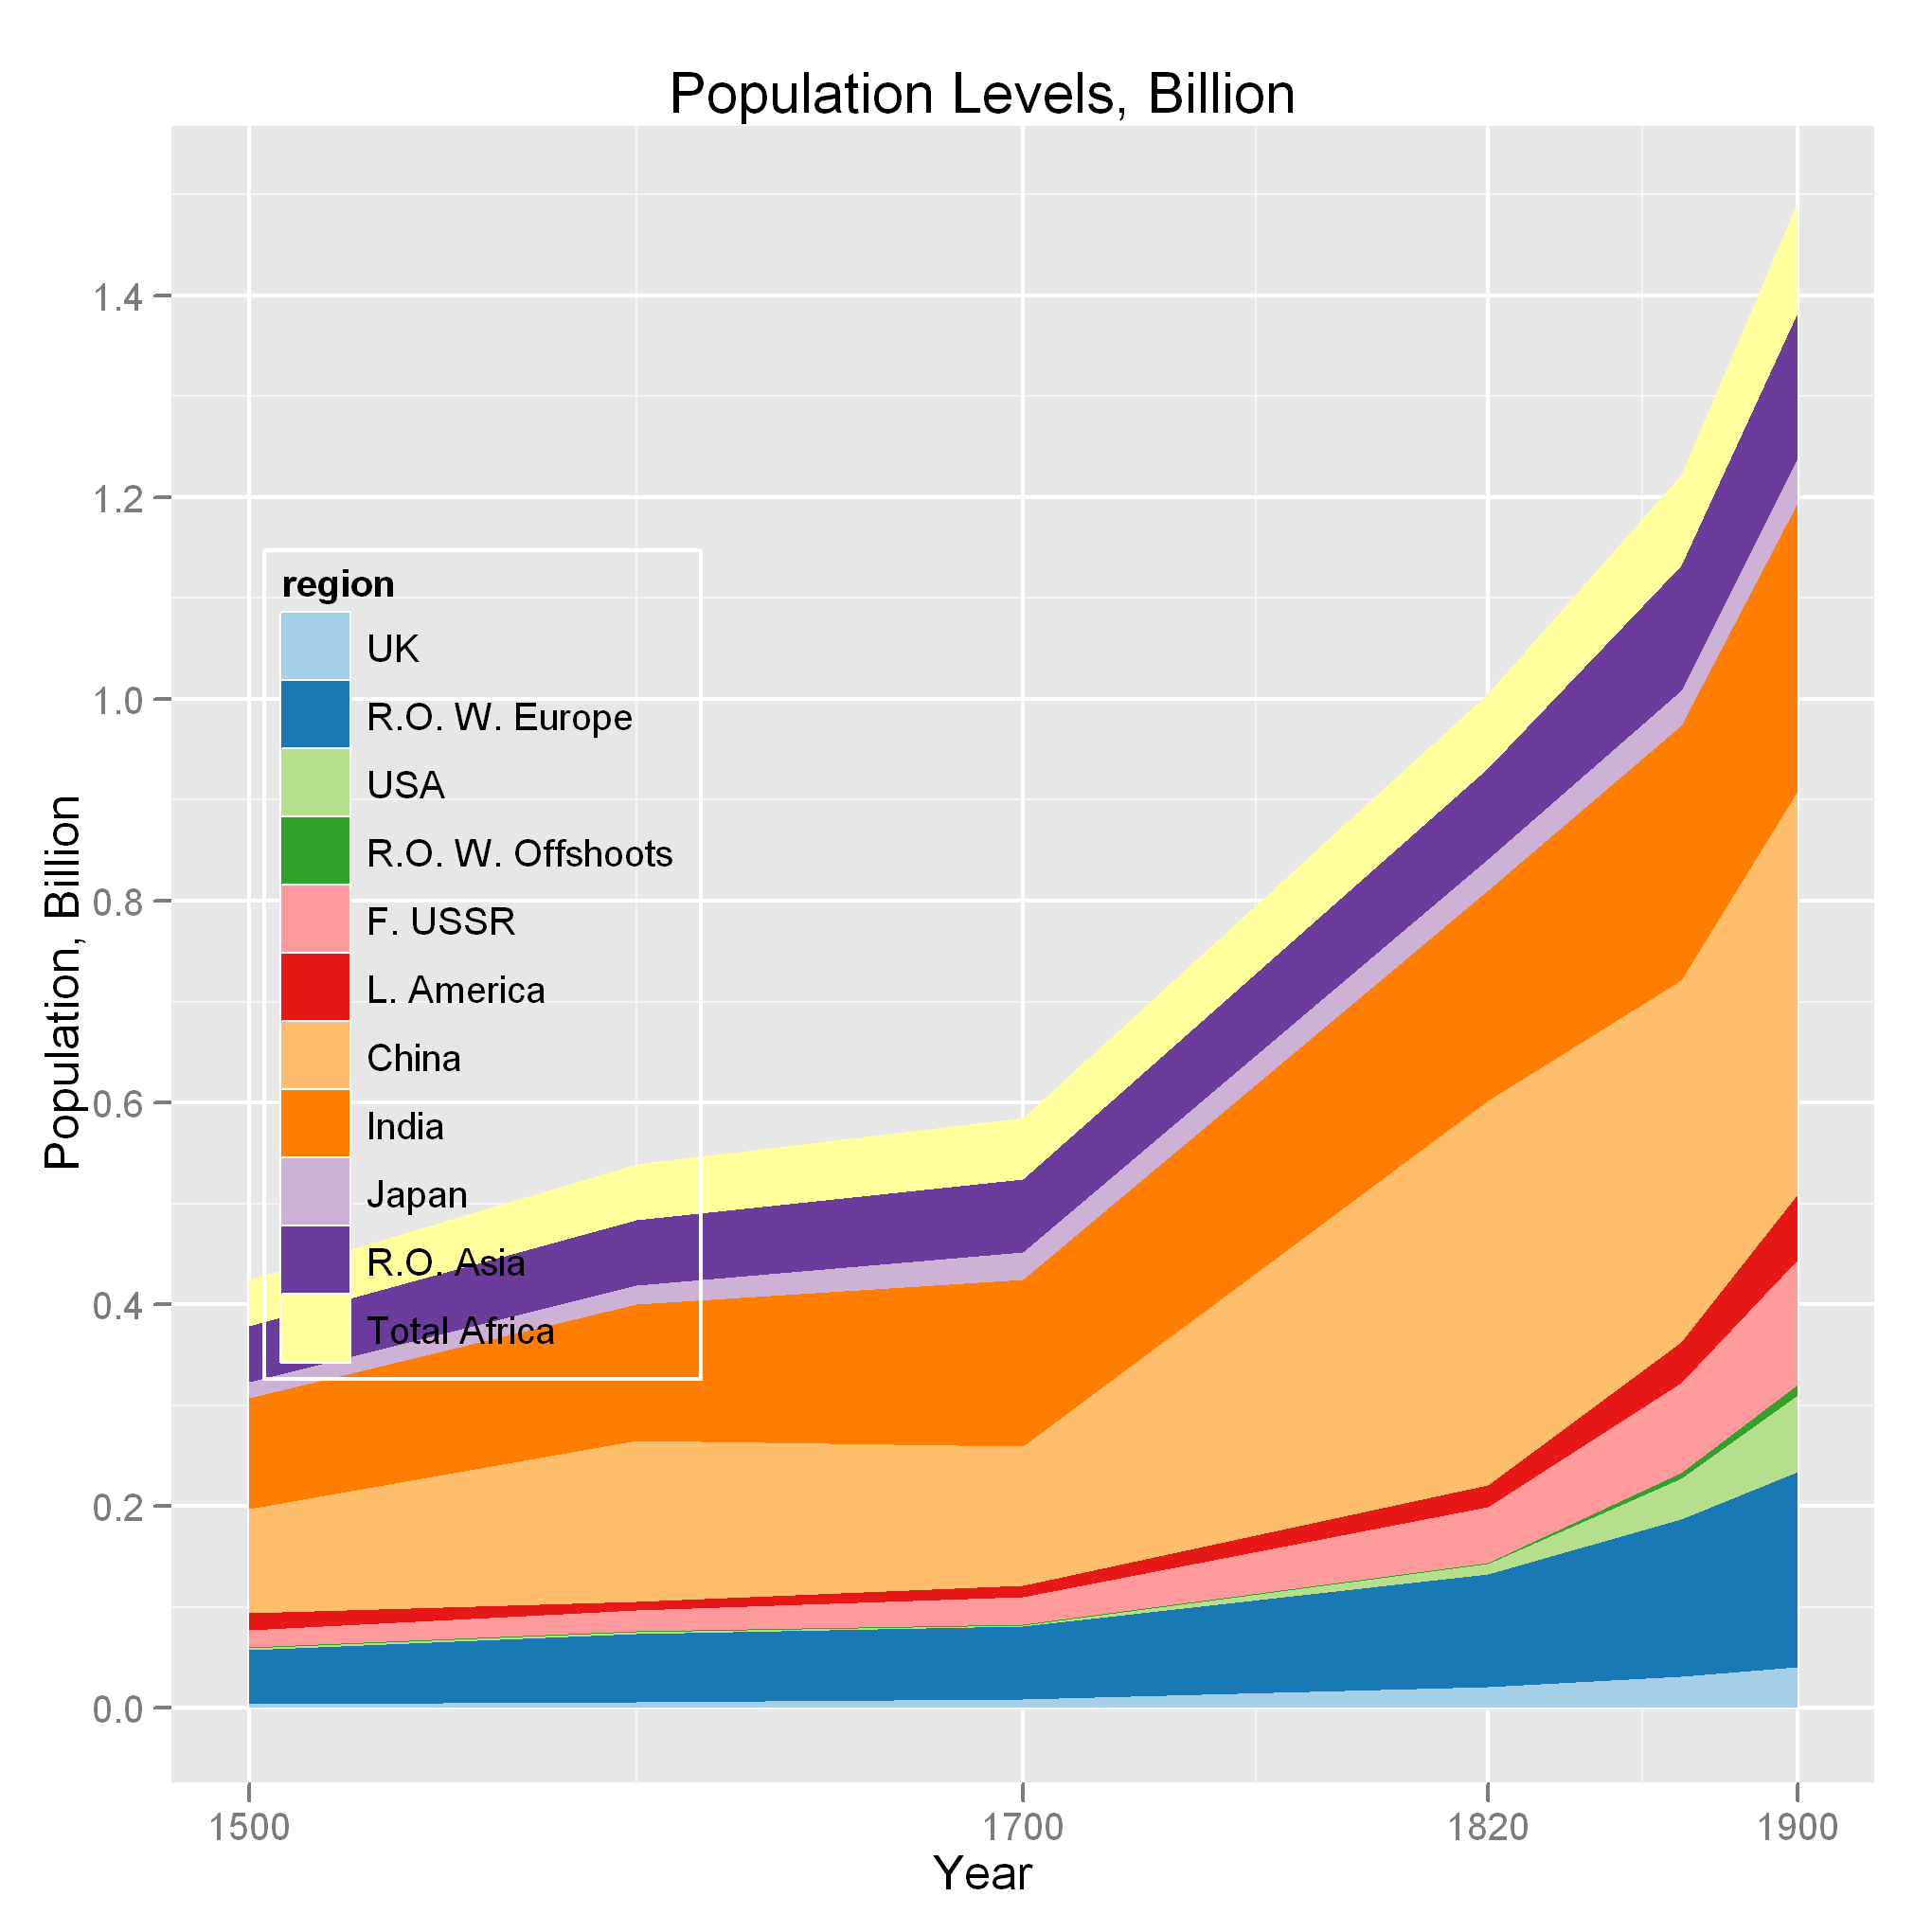
\includegraphics[width=0.60\textwidth]{maddisonregpoplevels1900.png}}
		\mbox{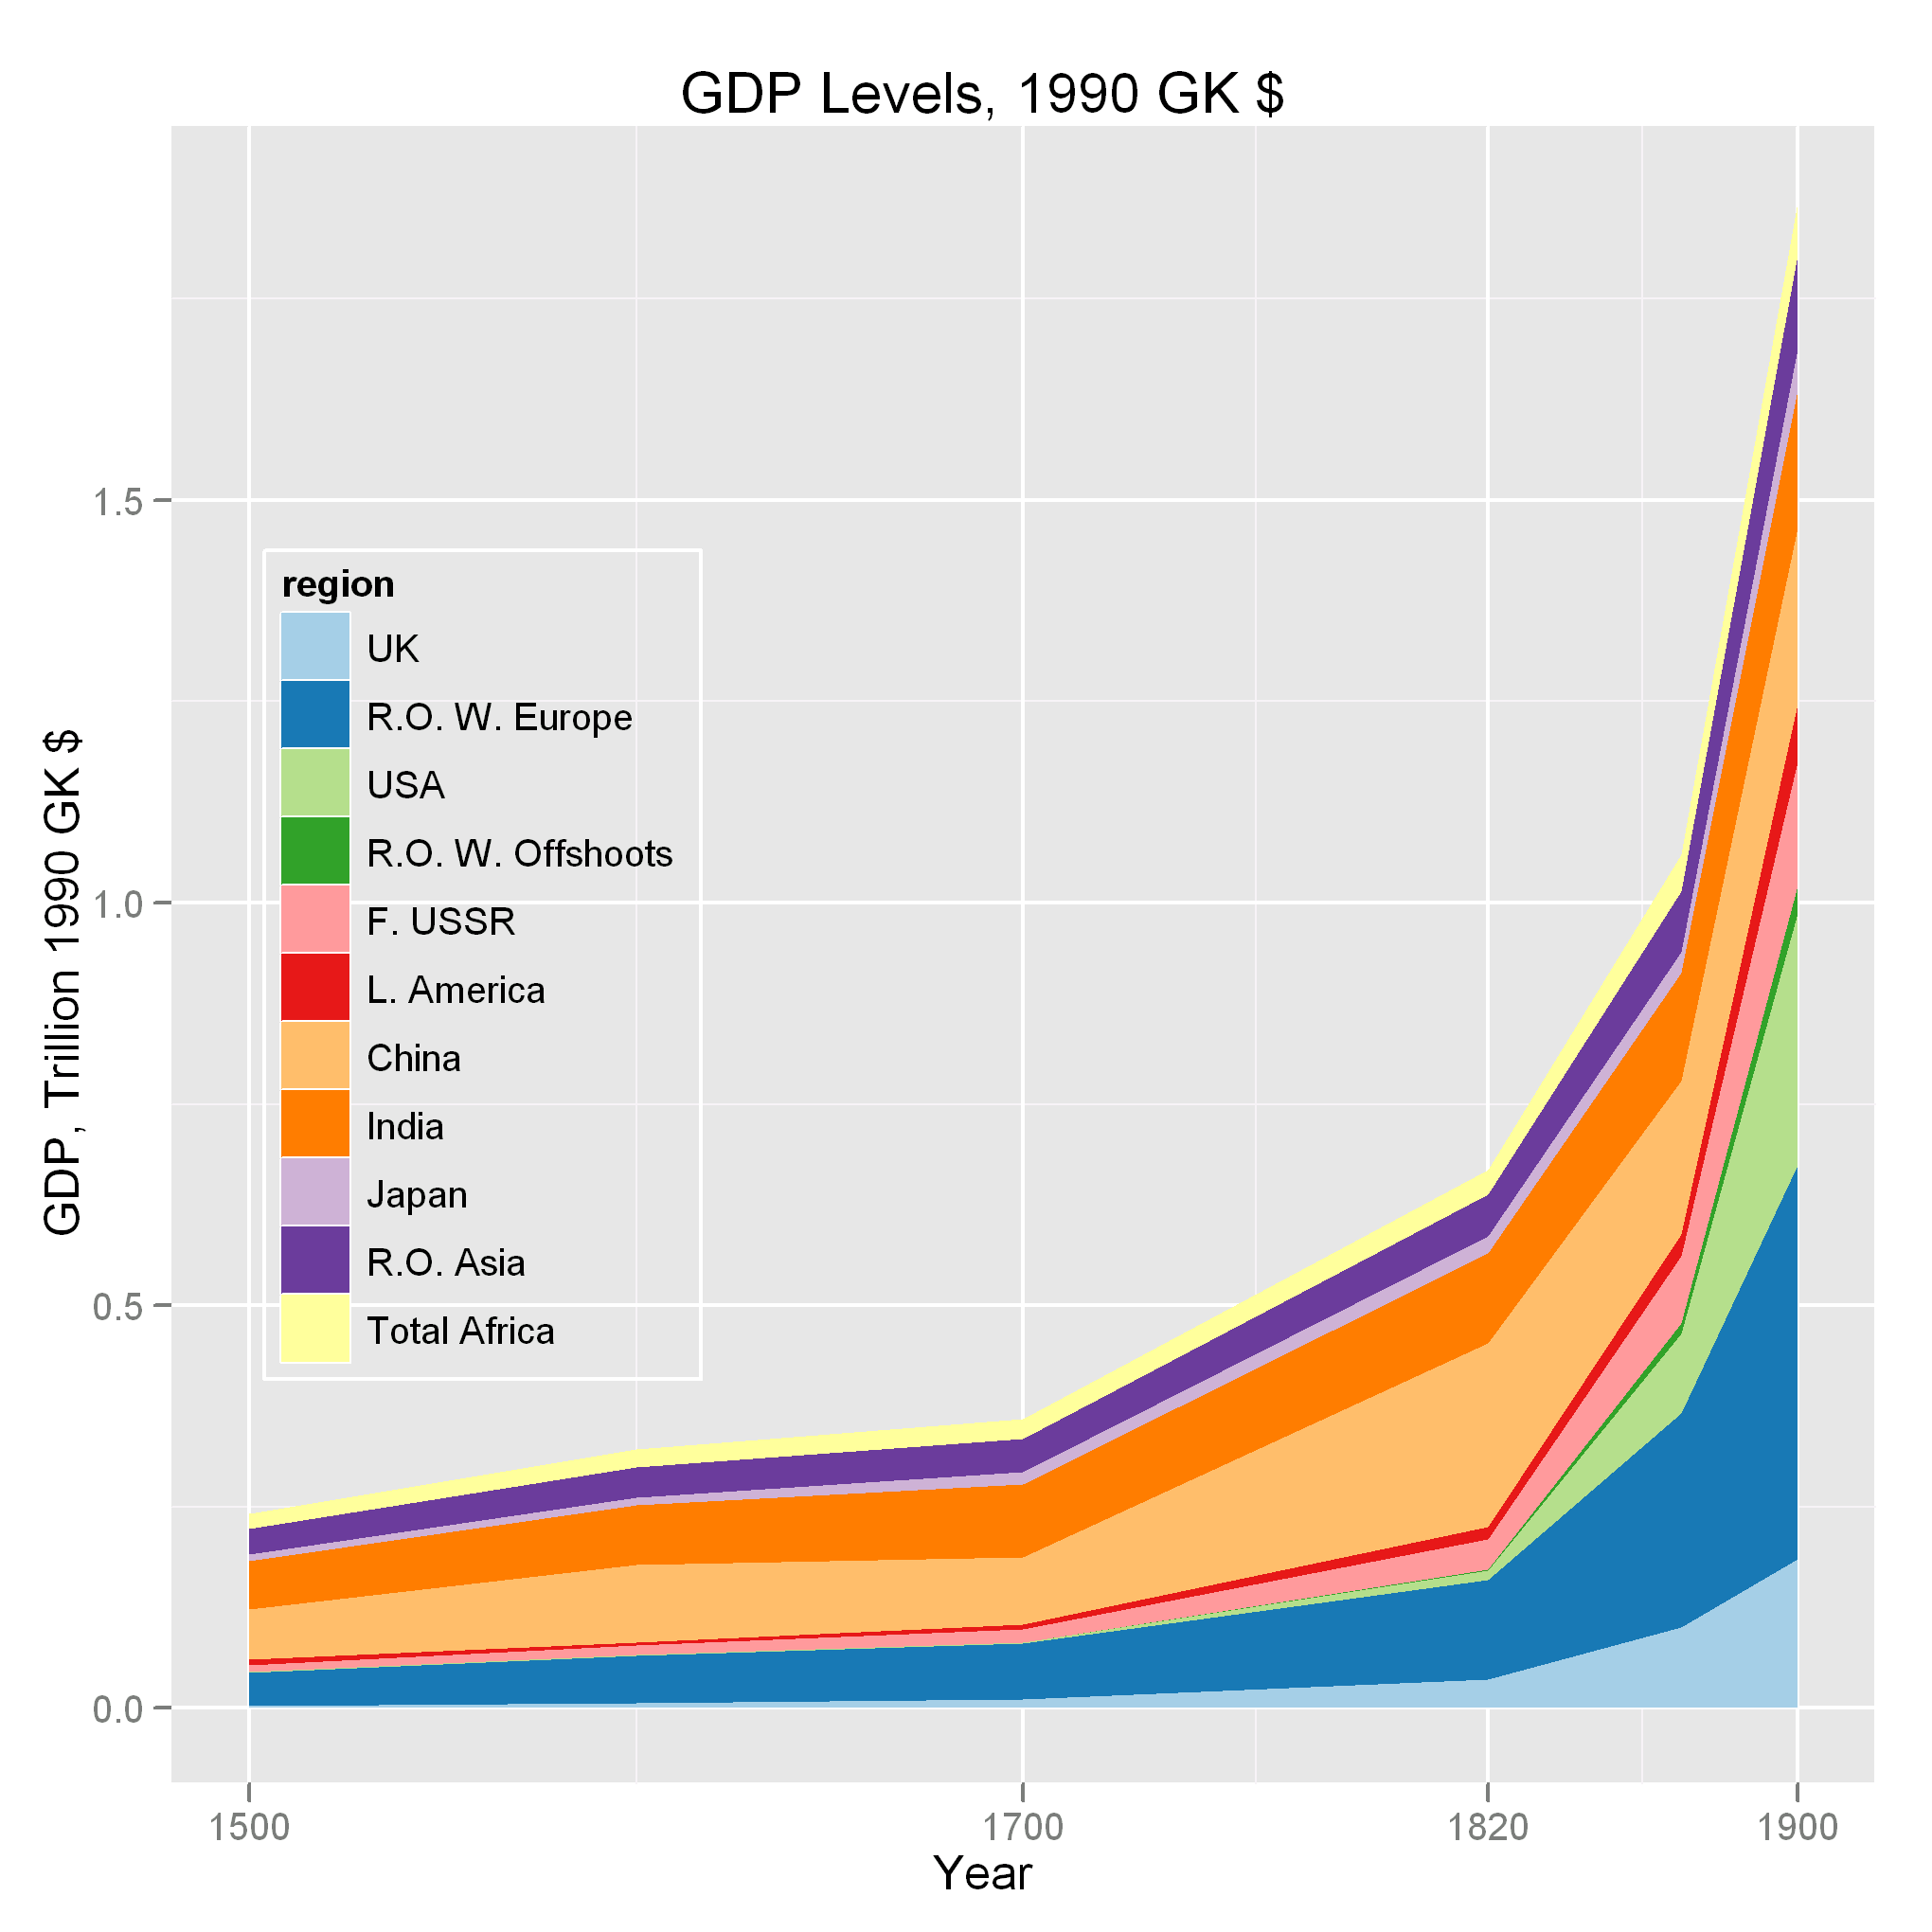
\includegraphics[width=0.60\textwidth]{maddisonreggdplevels1900.png}}
		}
		\caption{Angus Maddison: population and GDP levels 1500 -- 1900}
		\label{fig:poplevel1900}
		\end{figure}		
\end{frame}
\end{comment}

\subsection{Context -- Population and GDP proportions}	
\begin{frame}		
		\begin{figure}[h]
		\centerline{
		\mbox{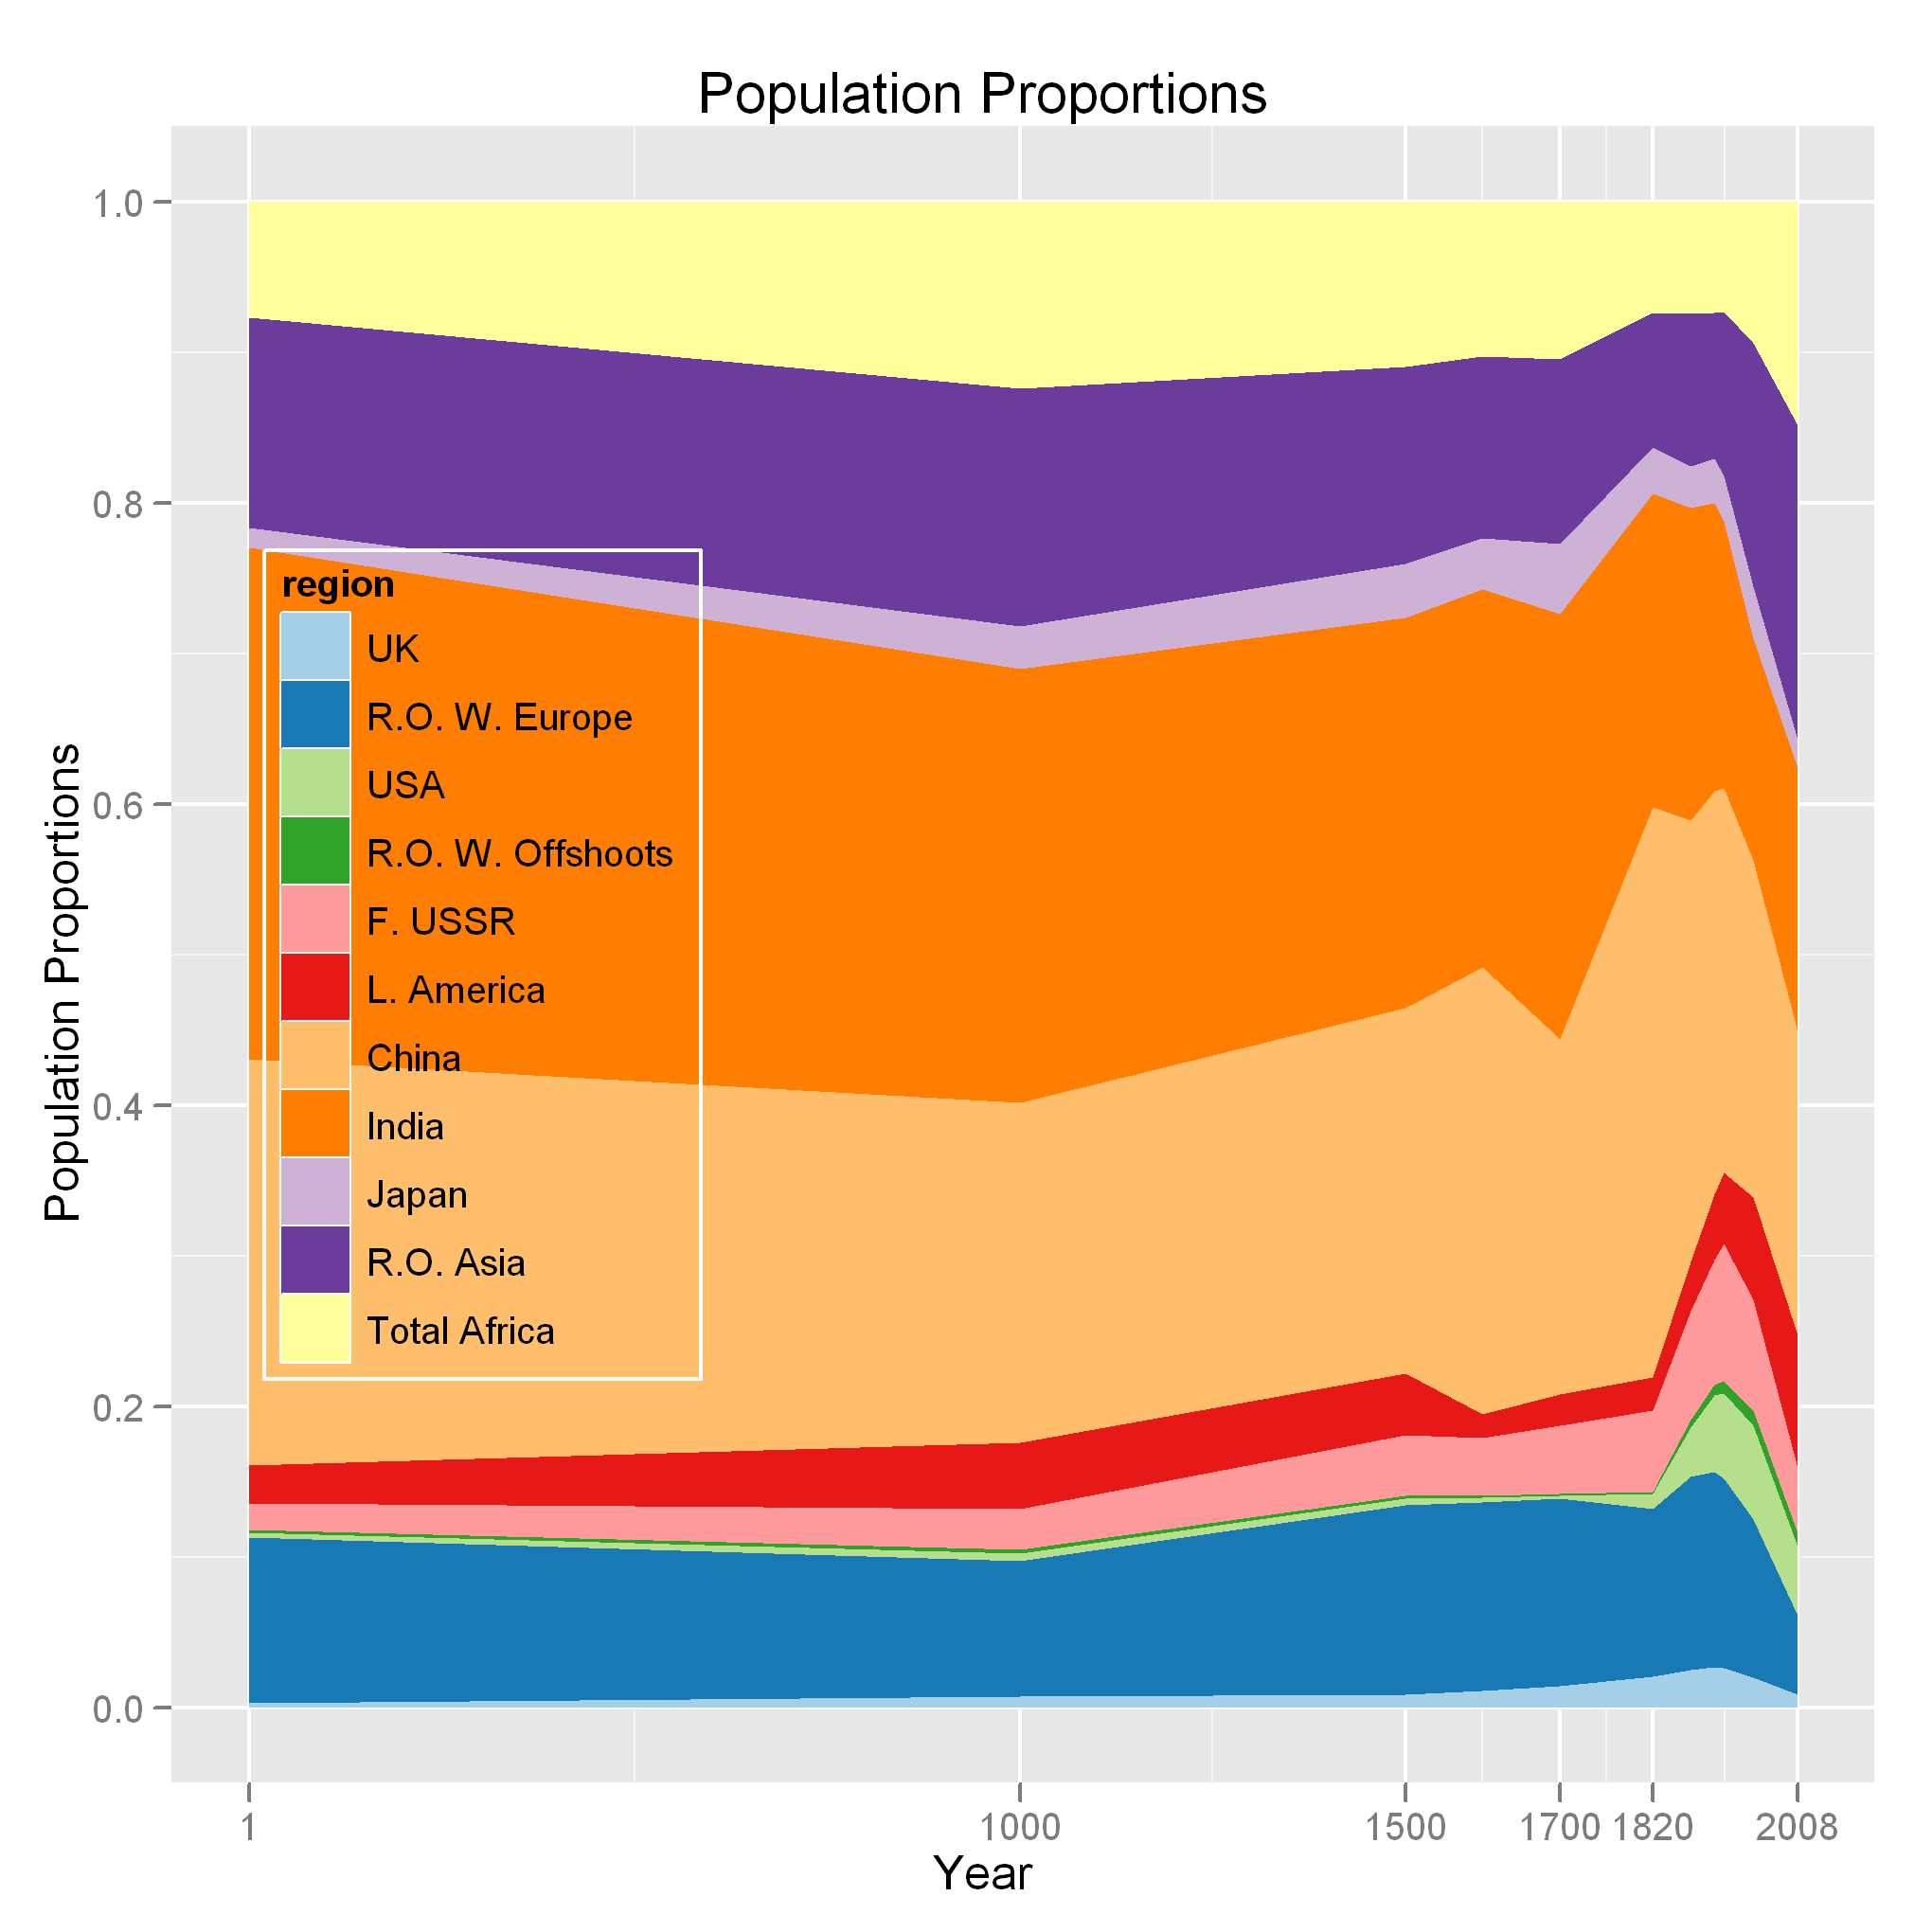
\includegraphics[width=0.58\textwidth]{maddisonregpoppct.png}}
		\mbox{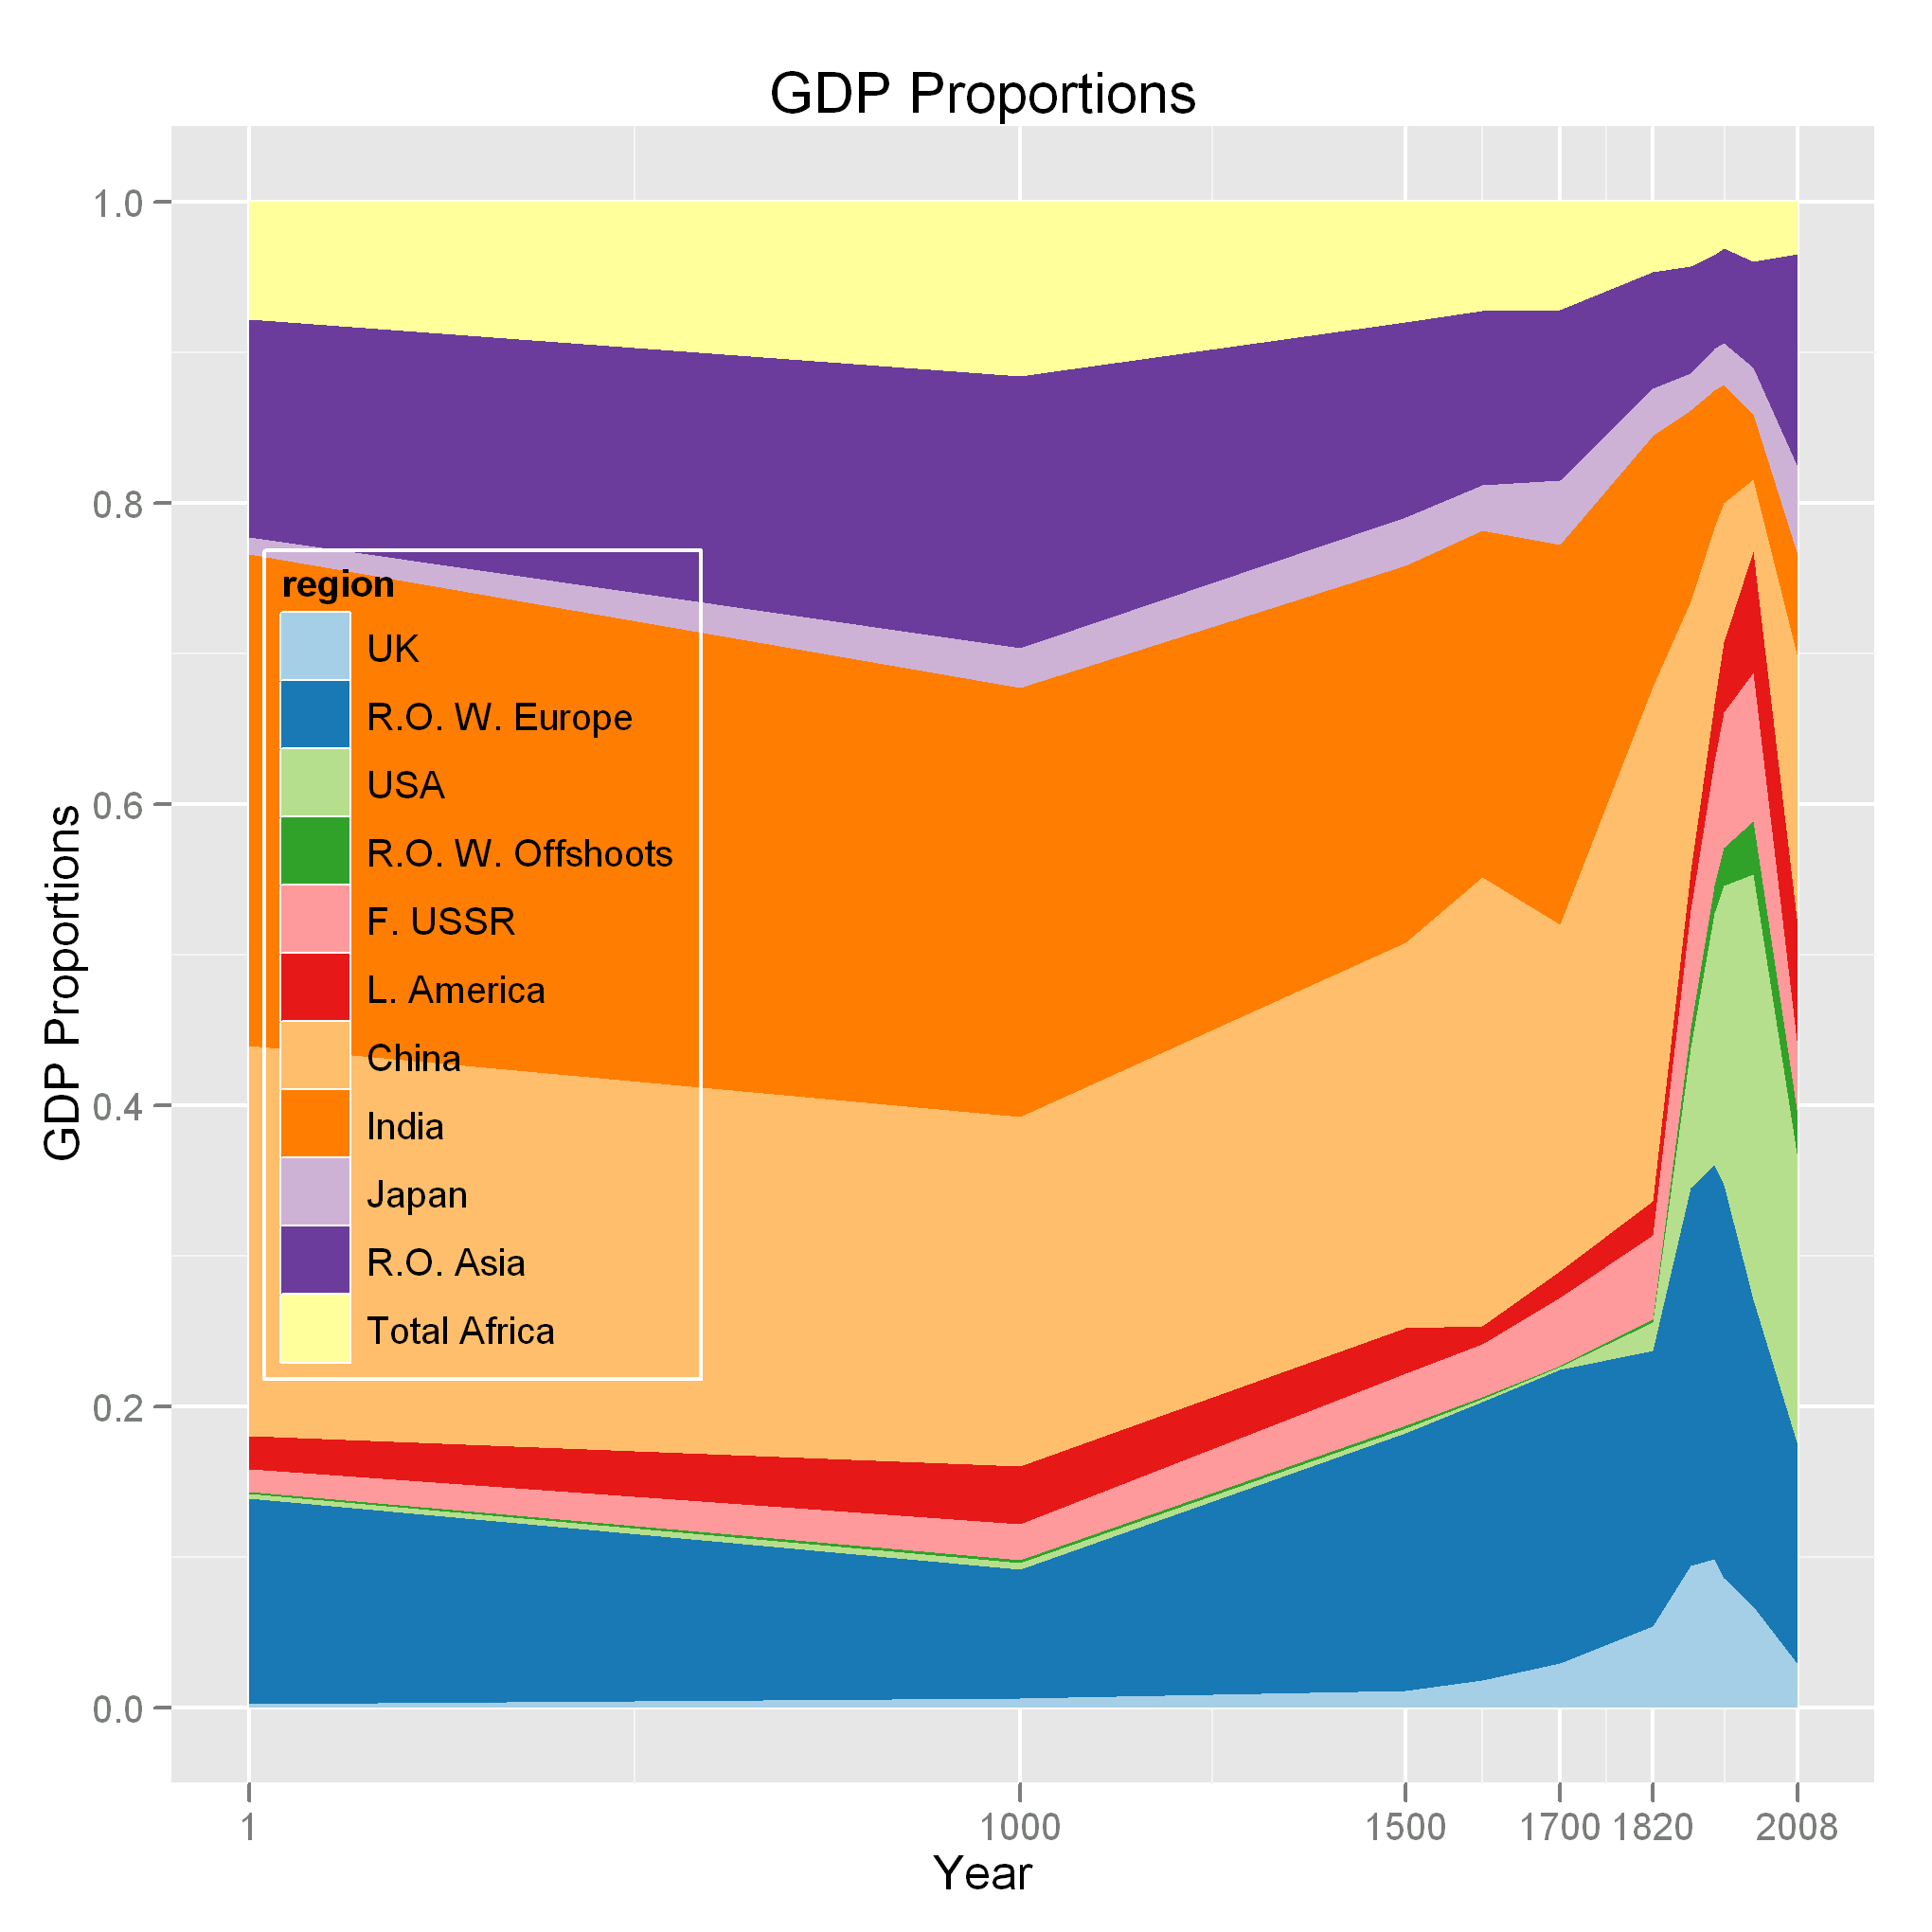
\includegraphics[width=0.58\textwidth]{maddisonreggdppct.png}}
		}
		\caption{Angus Maddison: population and GDP proportions CE 1 -- recent}
		\label{fig:poppct}
		\end{figure}	
\end{frame}

\subsection{Context -- Comparative growth 1500 -- current}
\begin{frame}
		\begin{figure}
		\centerline{
		\mbox{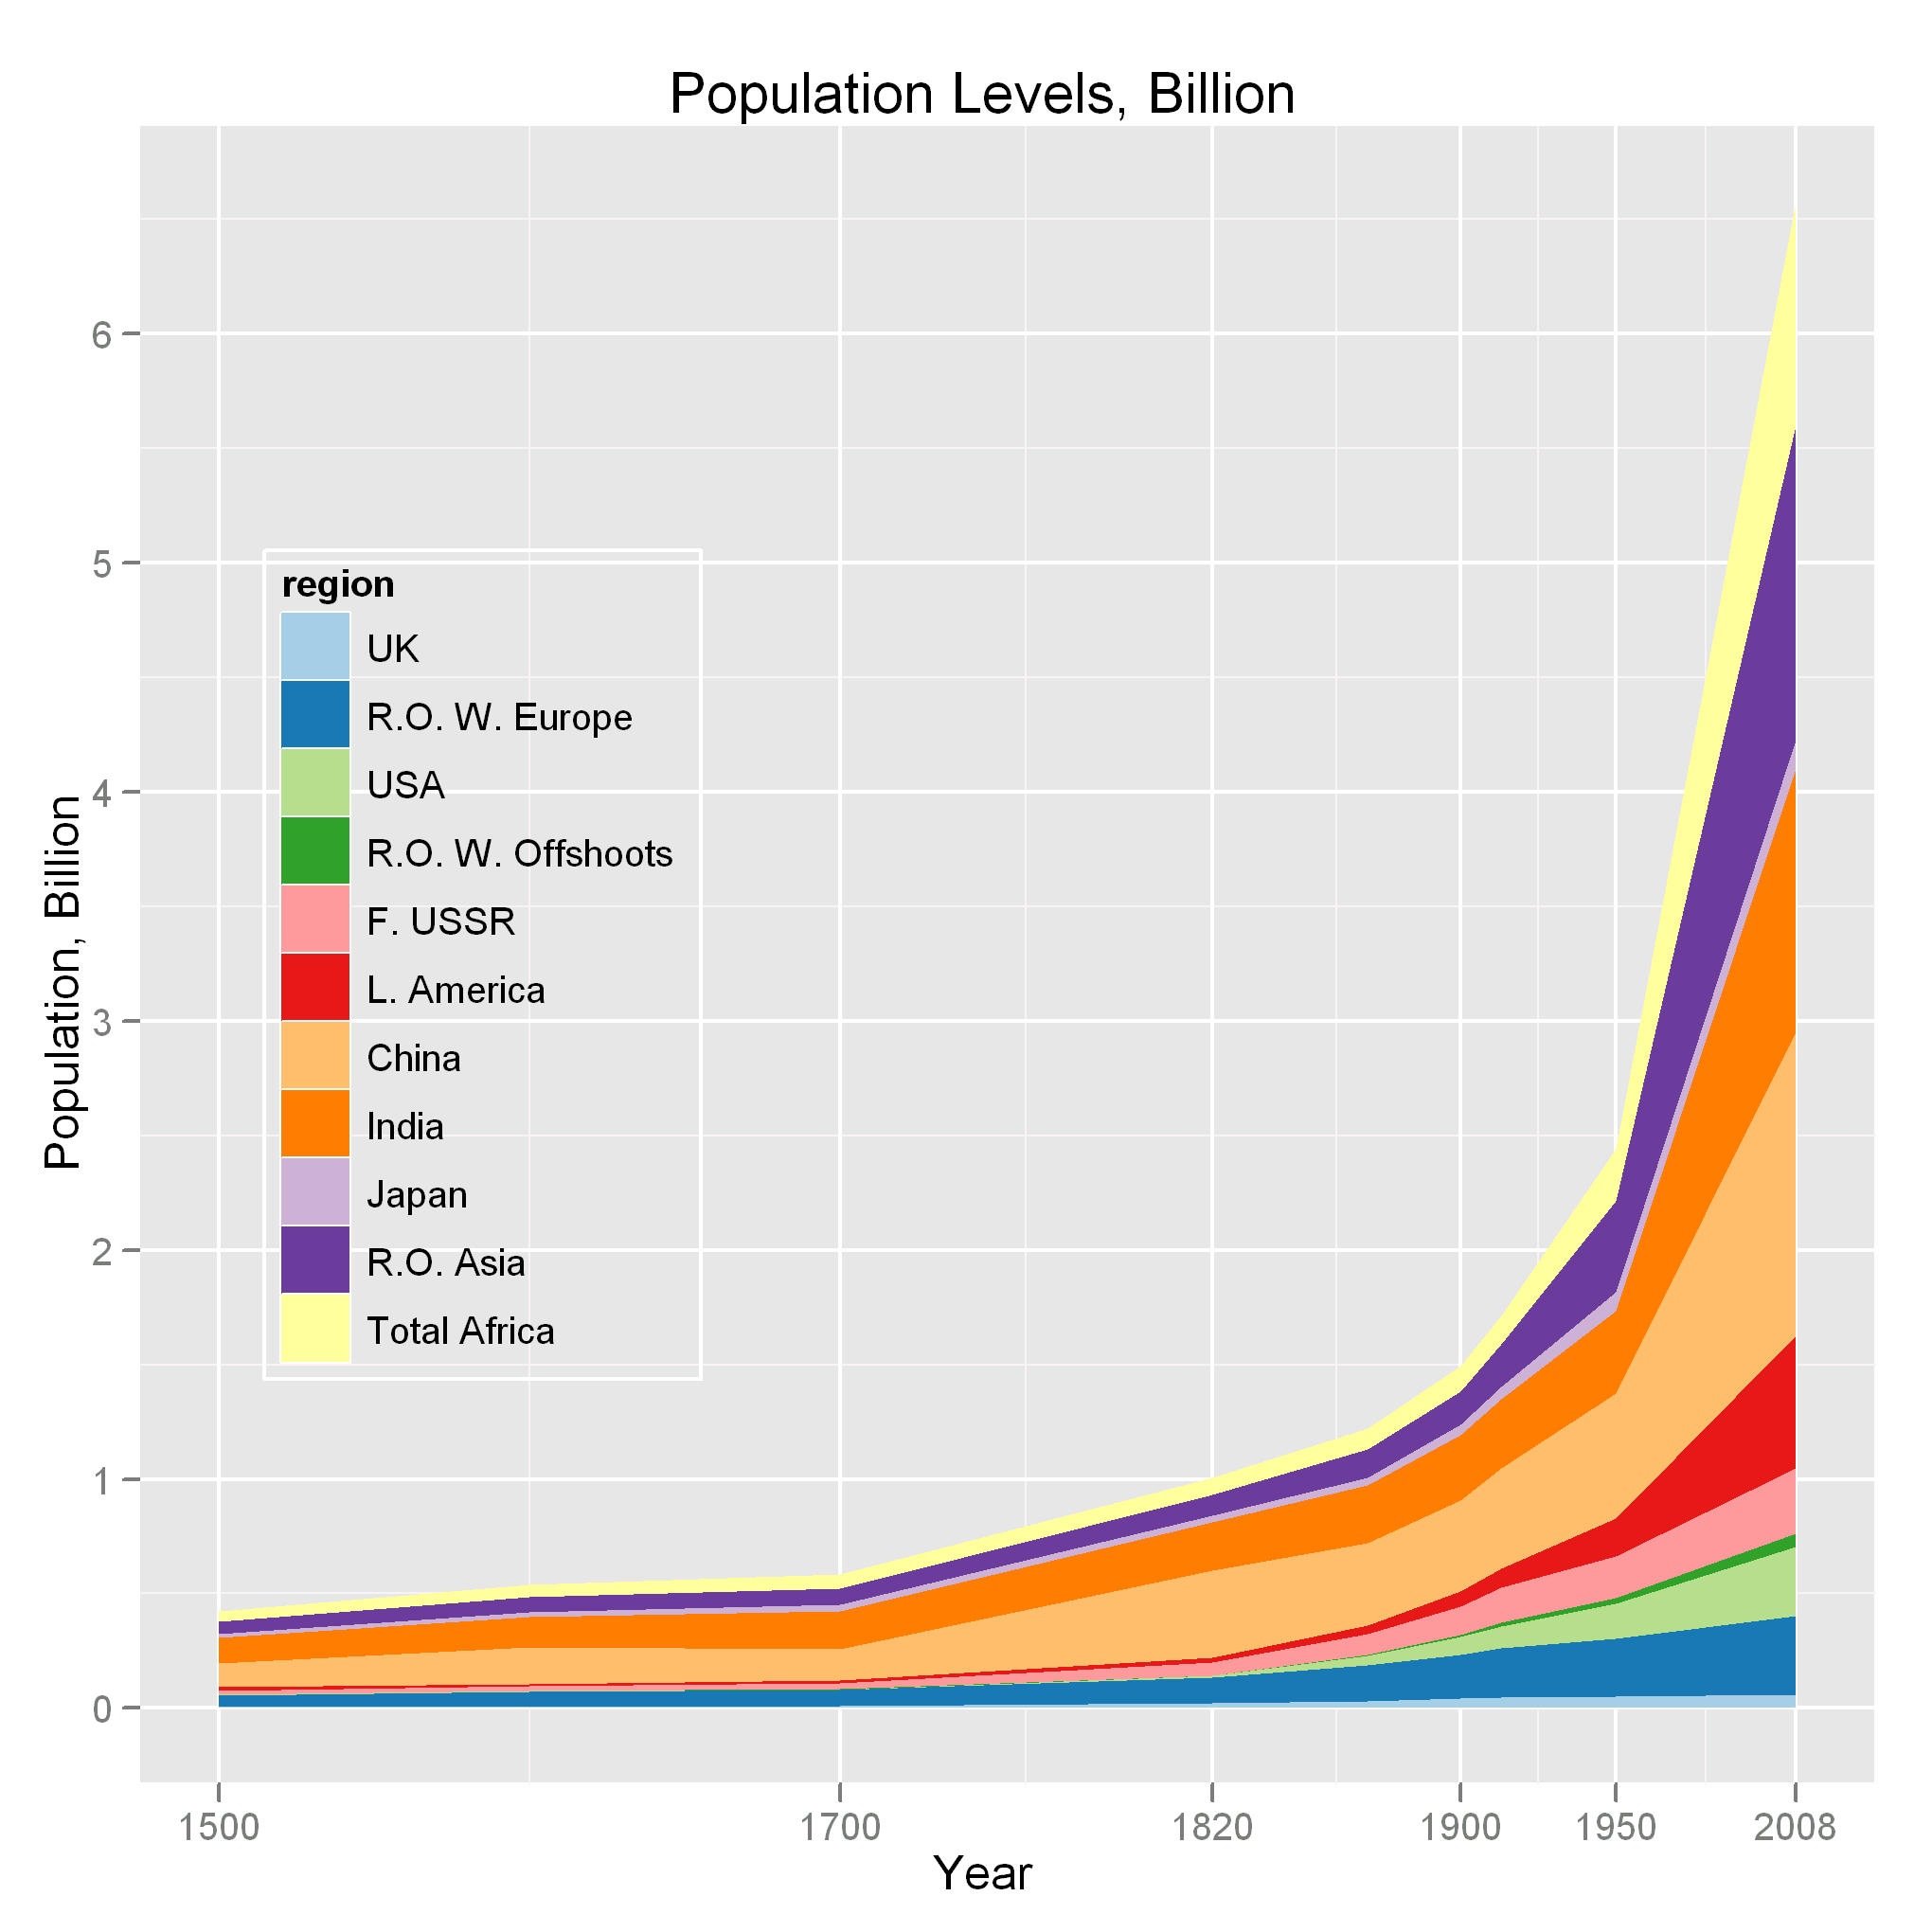
\includegraphics[width=0.58\textwidth]{maddisonregpoplevels.png}}
		\mbox{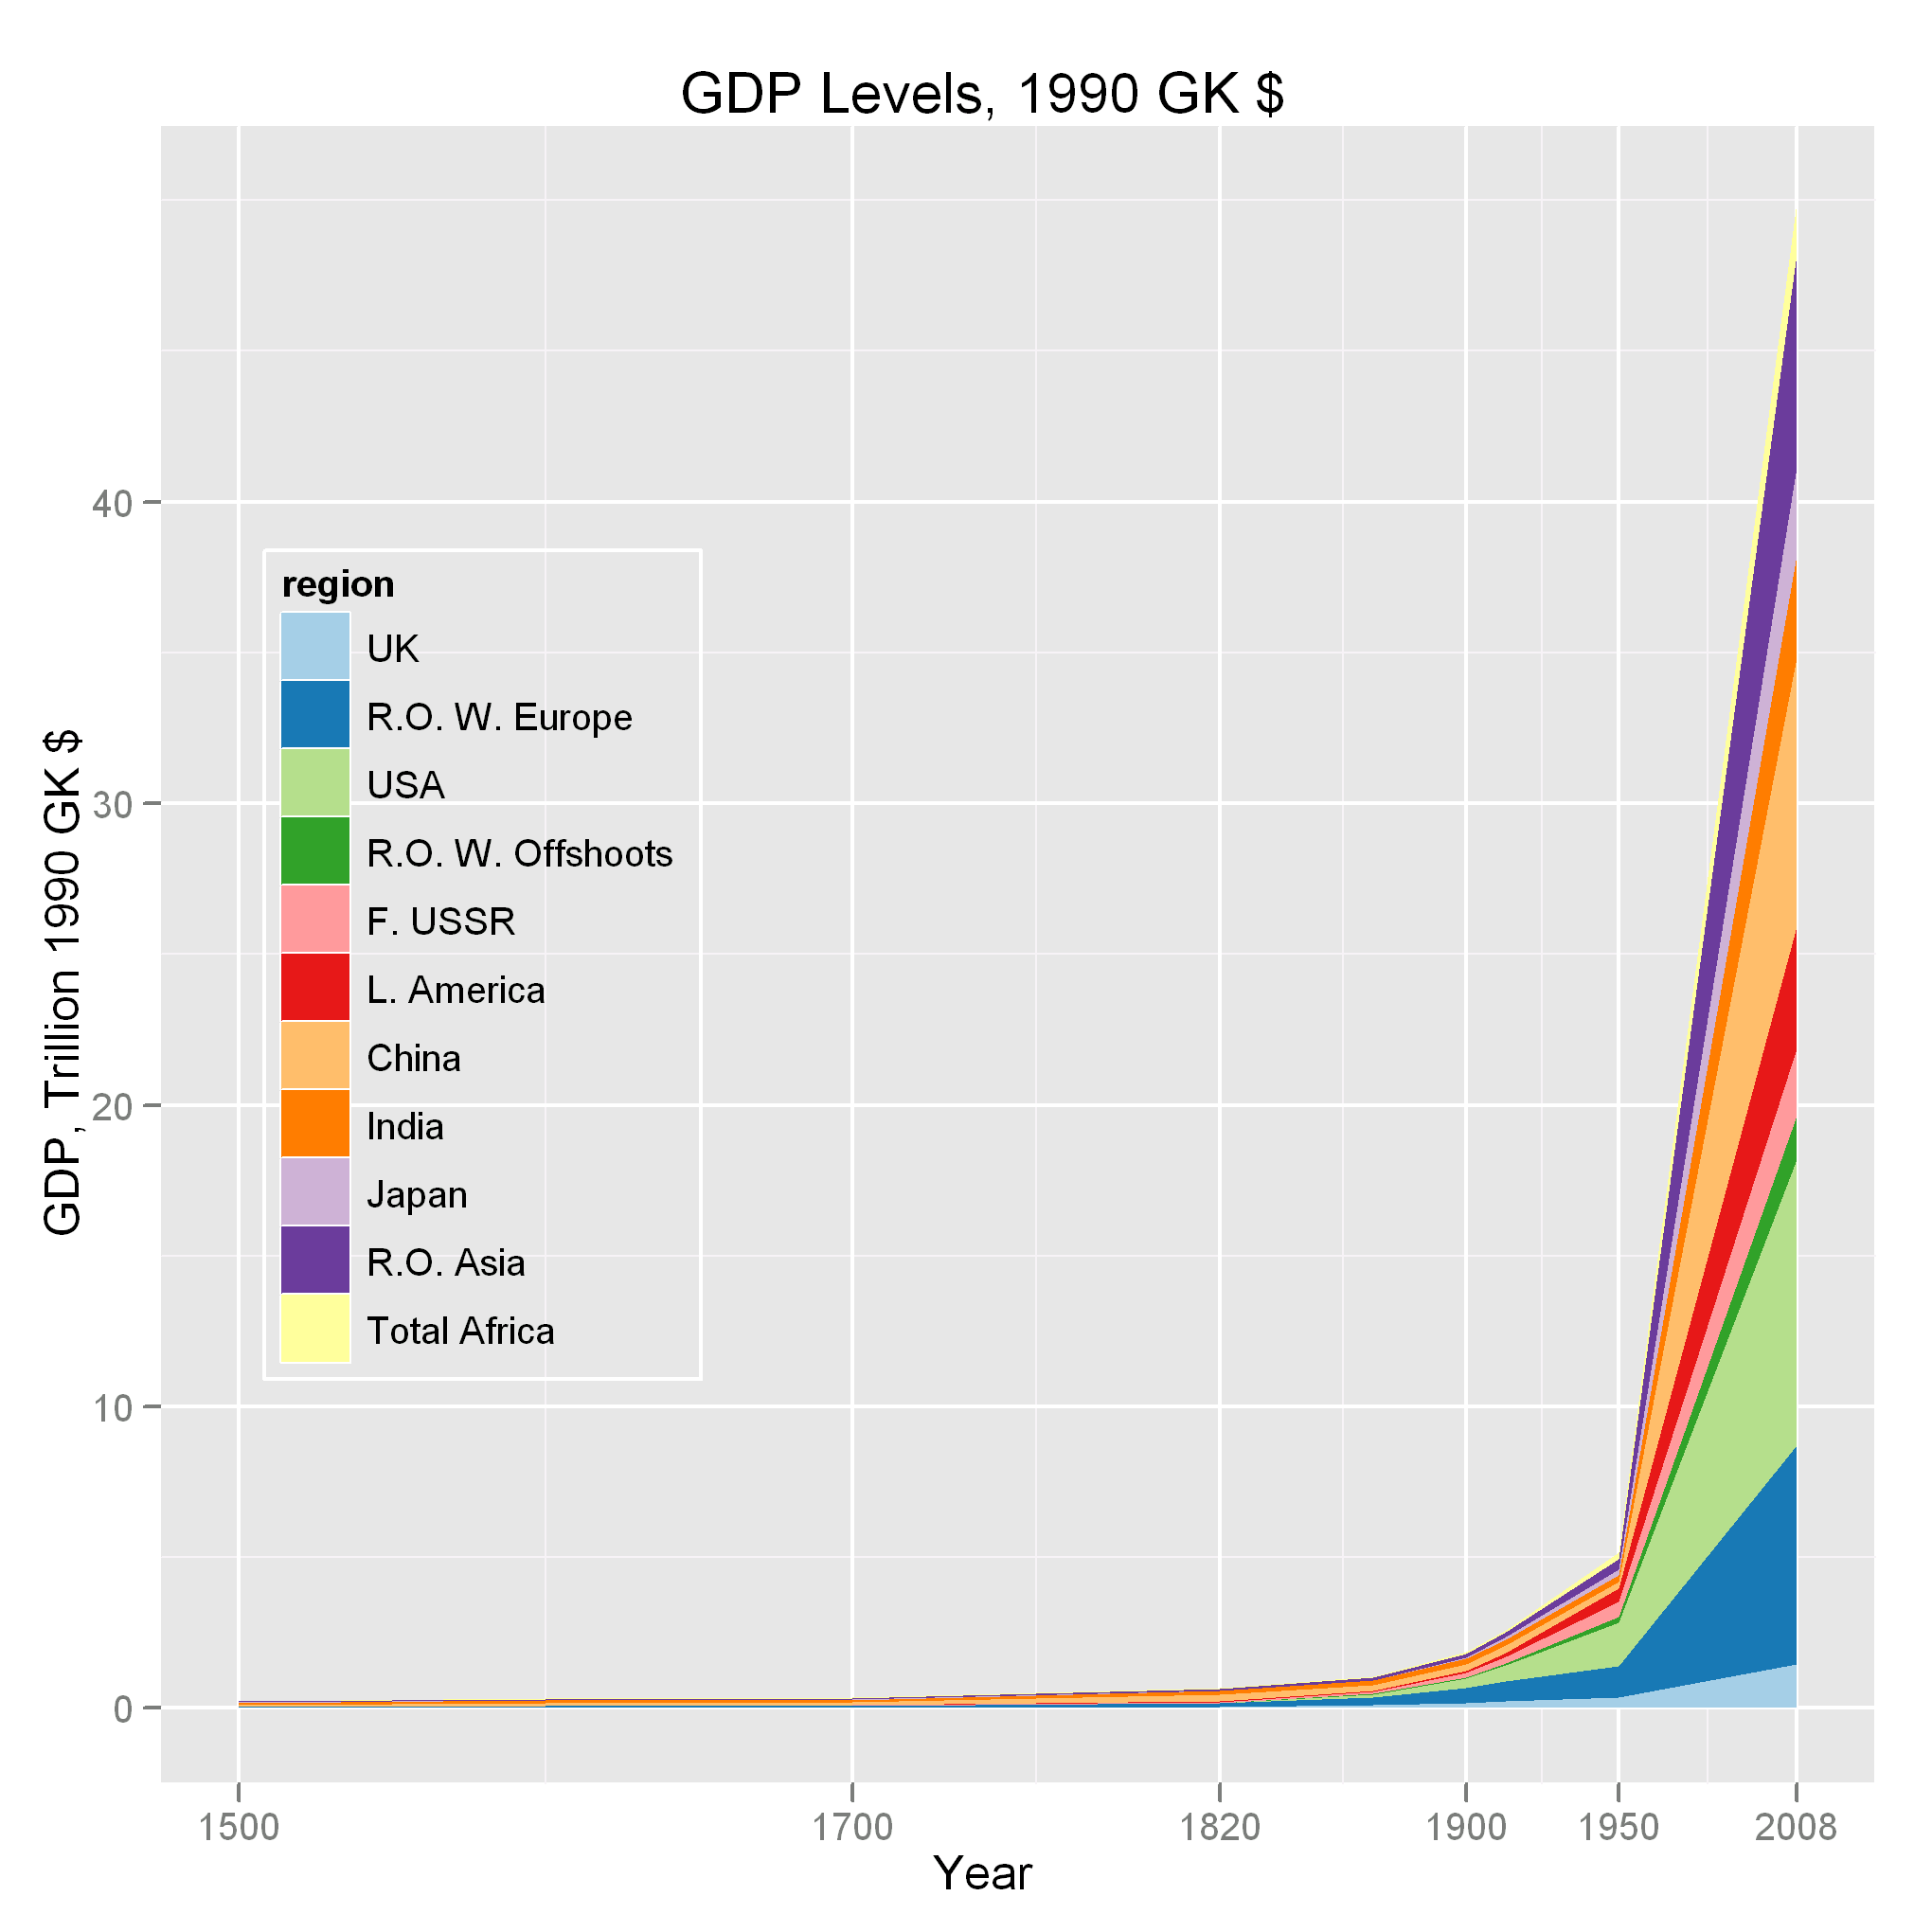
\includegraphics[width=0.58\textwidth]{maddisonreggdplevels.png}}
		}
		\caption{Angus Maddison: population and GDP levels 1500 through recent}
		\label{fig:poplevel}
		\end{figure}
		\footnote{Maddison, Angus. The World Economy: A Millennial Perspective/ Historical Statistics. Organization for Economic Cooperation \& Devel, 2007.}
\end{frame}




\subsection{The institutional case: China's sufficiency (Peer Vries)}
\begin{frame}
%\frametitle{The case: China's institutional sufficiency (Peer Vries)}

              \begin{itemize}

              	\item``Qing China was not a poor and static society but enjoyed a standard of living that was comparable to Europe's right through the early 1800s.''
				\item ``Chinese markets were both `much larger' and `closer to Smith's model of perfect competition than markets in Britain'.''
				\item ``China's foreign trade was `immense'.''
				\item ``Far from being ``despotic,'' the Chinese Qing state was even less intrusive than Britain's: not only was the Chinese army `comparatively small' but Britain had `more than 30 times as many public servants per head of the population,' plus Chinese taxes seem to have been lower.''
 just as little, an 'open society' as Britain was'.''
				               \footnote{Vries, Peer.``Is California the Measure of All Things Global? A Rejoinder to Ricardo Duchesne, `Peer Vries, the Great Divergence, and the California School: Who's in and Who's Out.'' World History Connected 2, no. 2 (May 2005). http://worldhistoryconnected.press.illinois.edu/2.2/vries.html.}

				\end{itemize}
\end{frame}

\begin{frame}
%\frametitle{The case: China's institutional sufficiency (Peer Vries), continued }
              \begin{itemize}				
				\item ``China in the eighteenth and nineteenth centuries, in terms of social mobility, `was just as much, or if you prefer,
				\item ``Weber was wrong: Chinese `rationality, work ethos, business acumen, and love of profit' were just as vivid as in Britain.''
				\item ''As late as the end of the eighteenth century, China's agriculture per hectare still was much more productive than Britain's agriculture; in terms of productivity per labourer the differences between both countries or their core regions were minimal.''
				\item ``BUT \ldots China's economy was not moving away from the Malthusian limitations of the old regime, and was not as ready to industrialize as England.''
				\item Pomeranz and Wong (and others) support this point of view -- essentially saying that Europe had no sufficiently special institutions to explain history.
				
				\end{itemize}
\end{frame}		


\subsection{Why England did it -- why China did not}

\begin{frame}
\frametitle{The microeconomics of energy source substitution} 	
 		\begin{figure}
		\centerline{
		\mbox{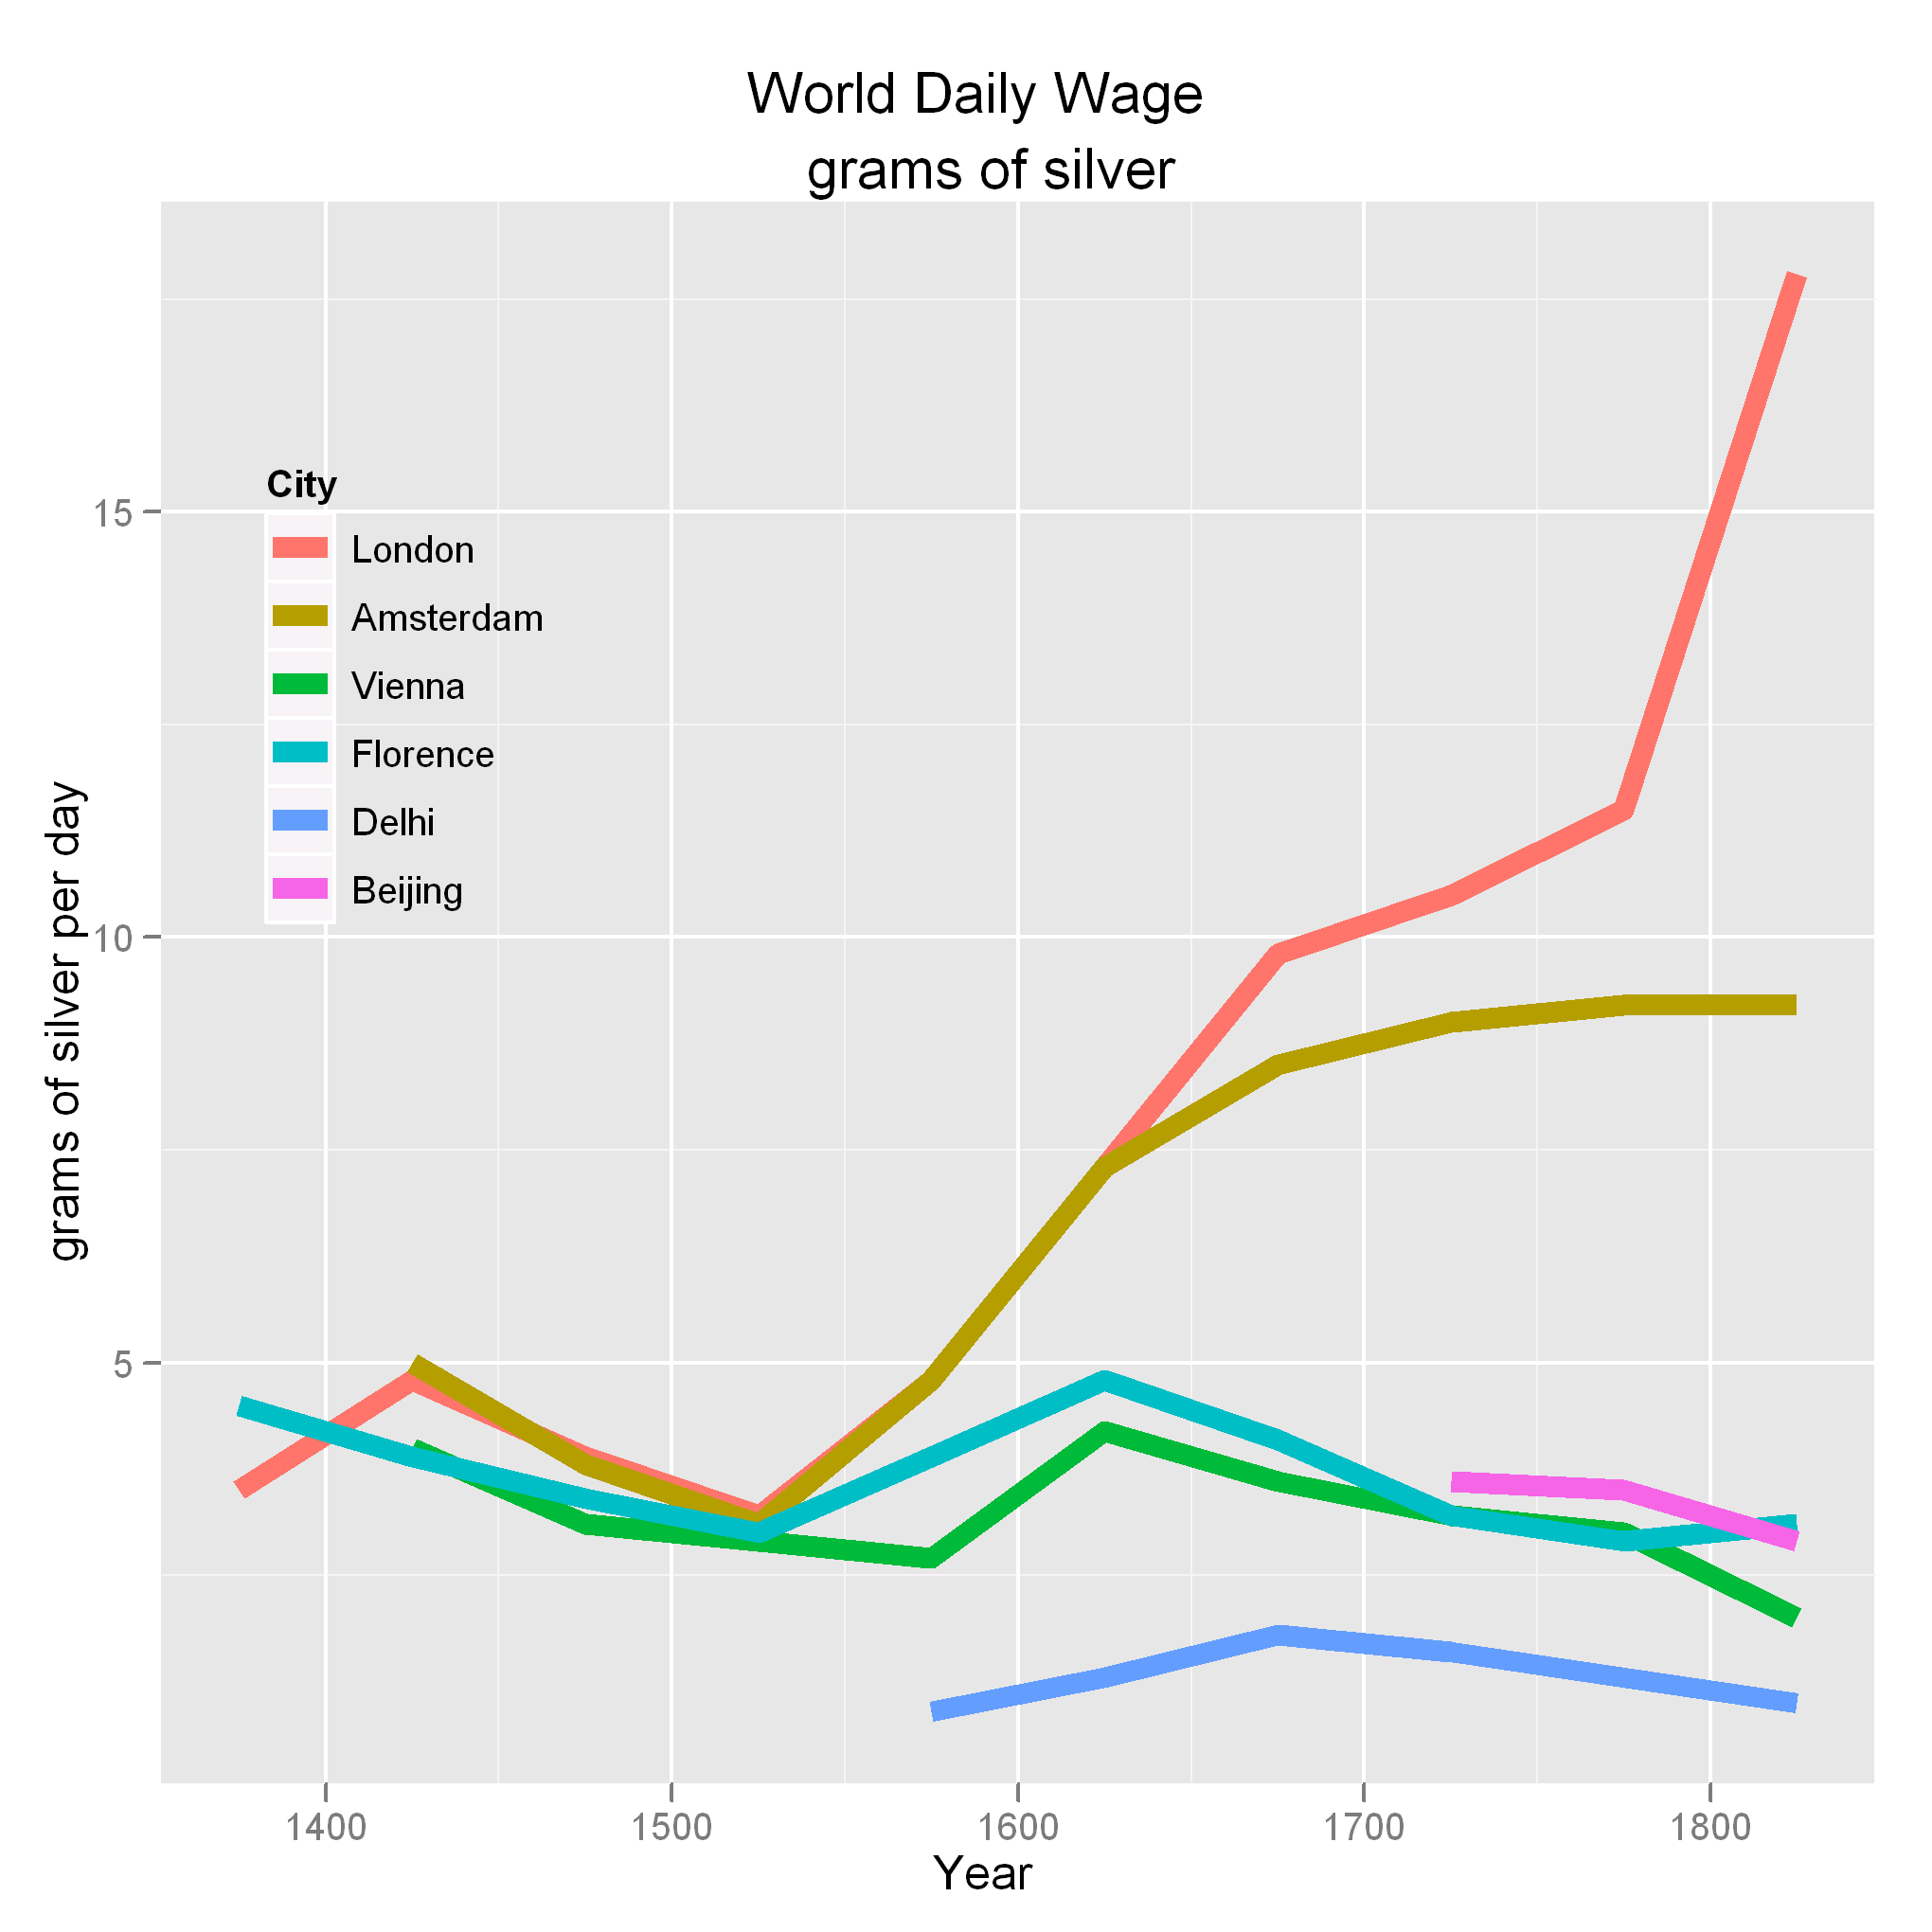
\includegraphics[width=0.39\textwidth]{gworldwages.png}}
		\mbox{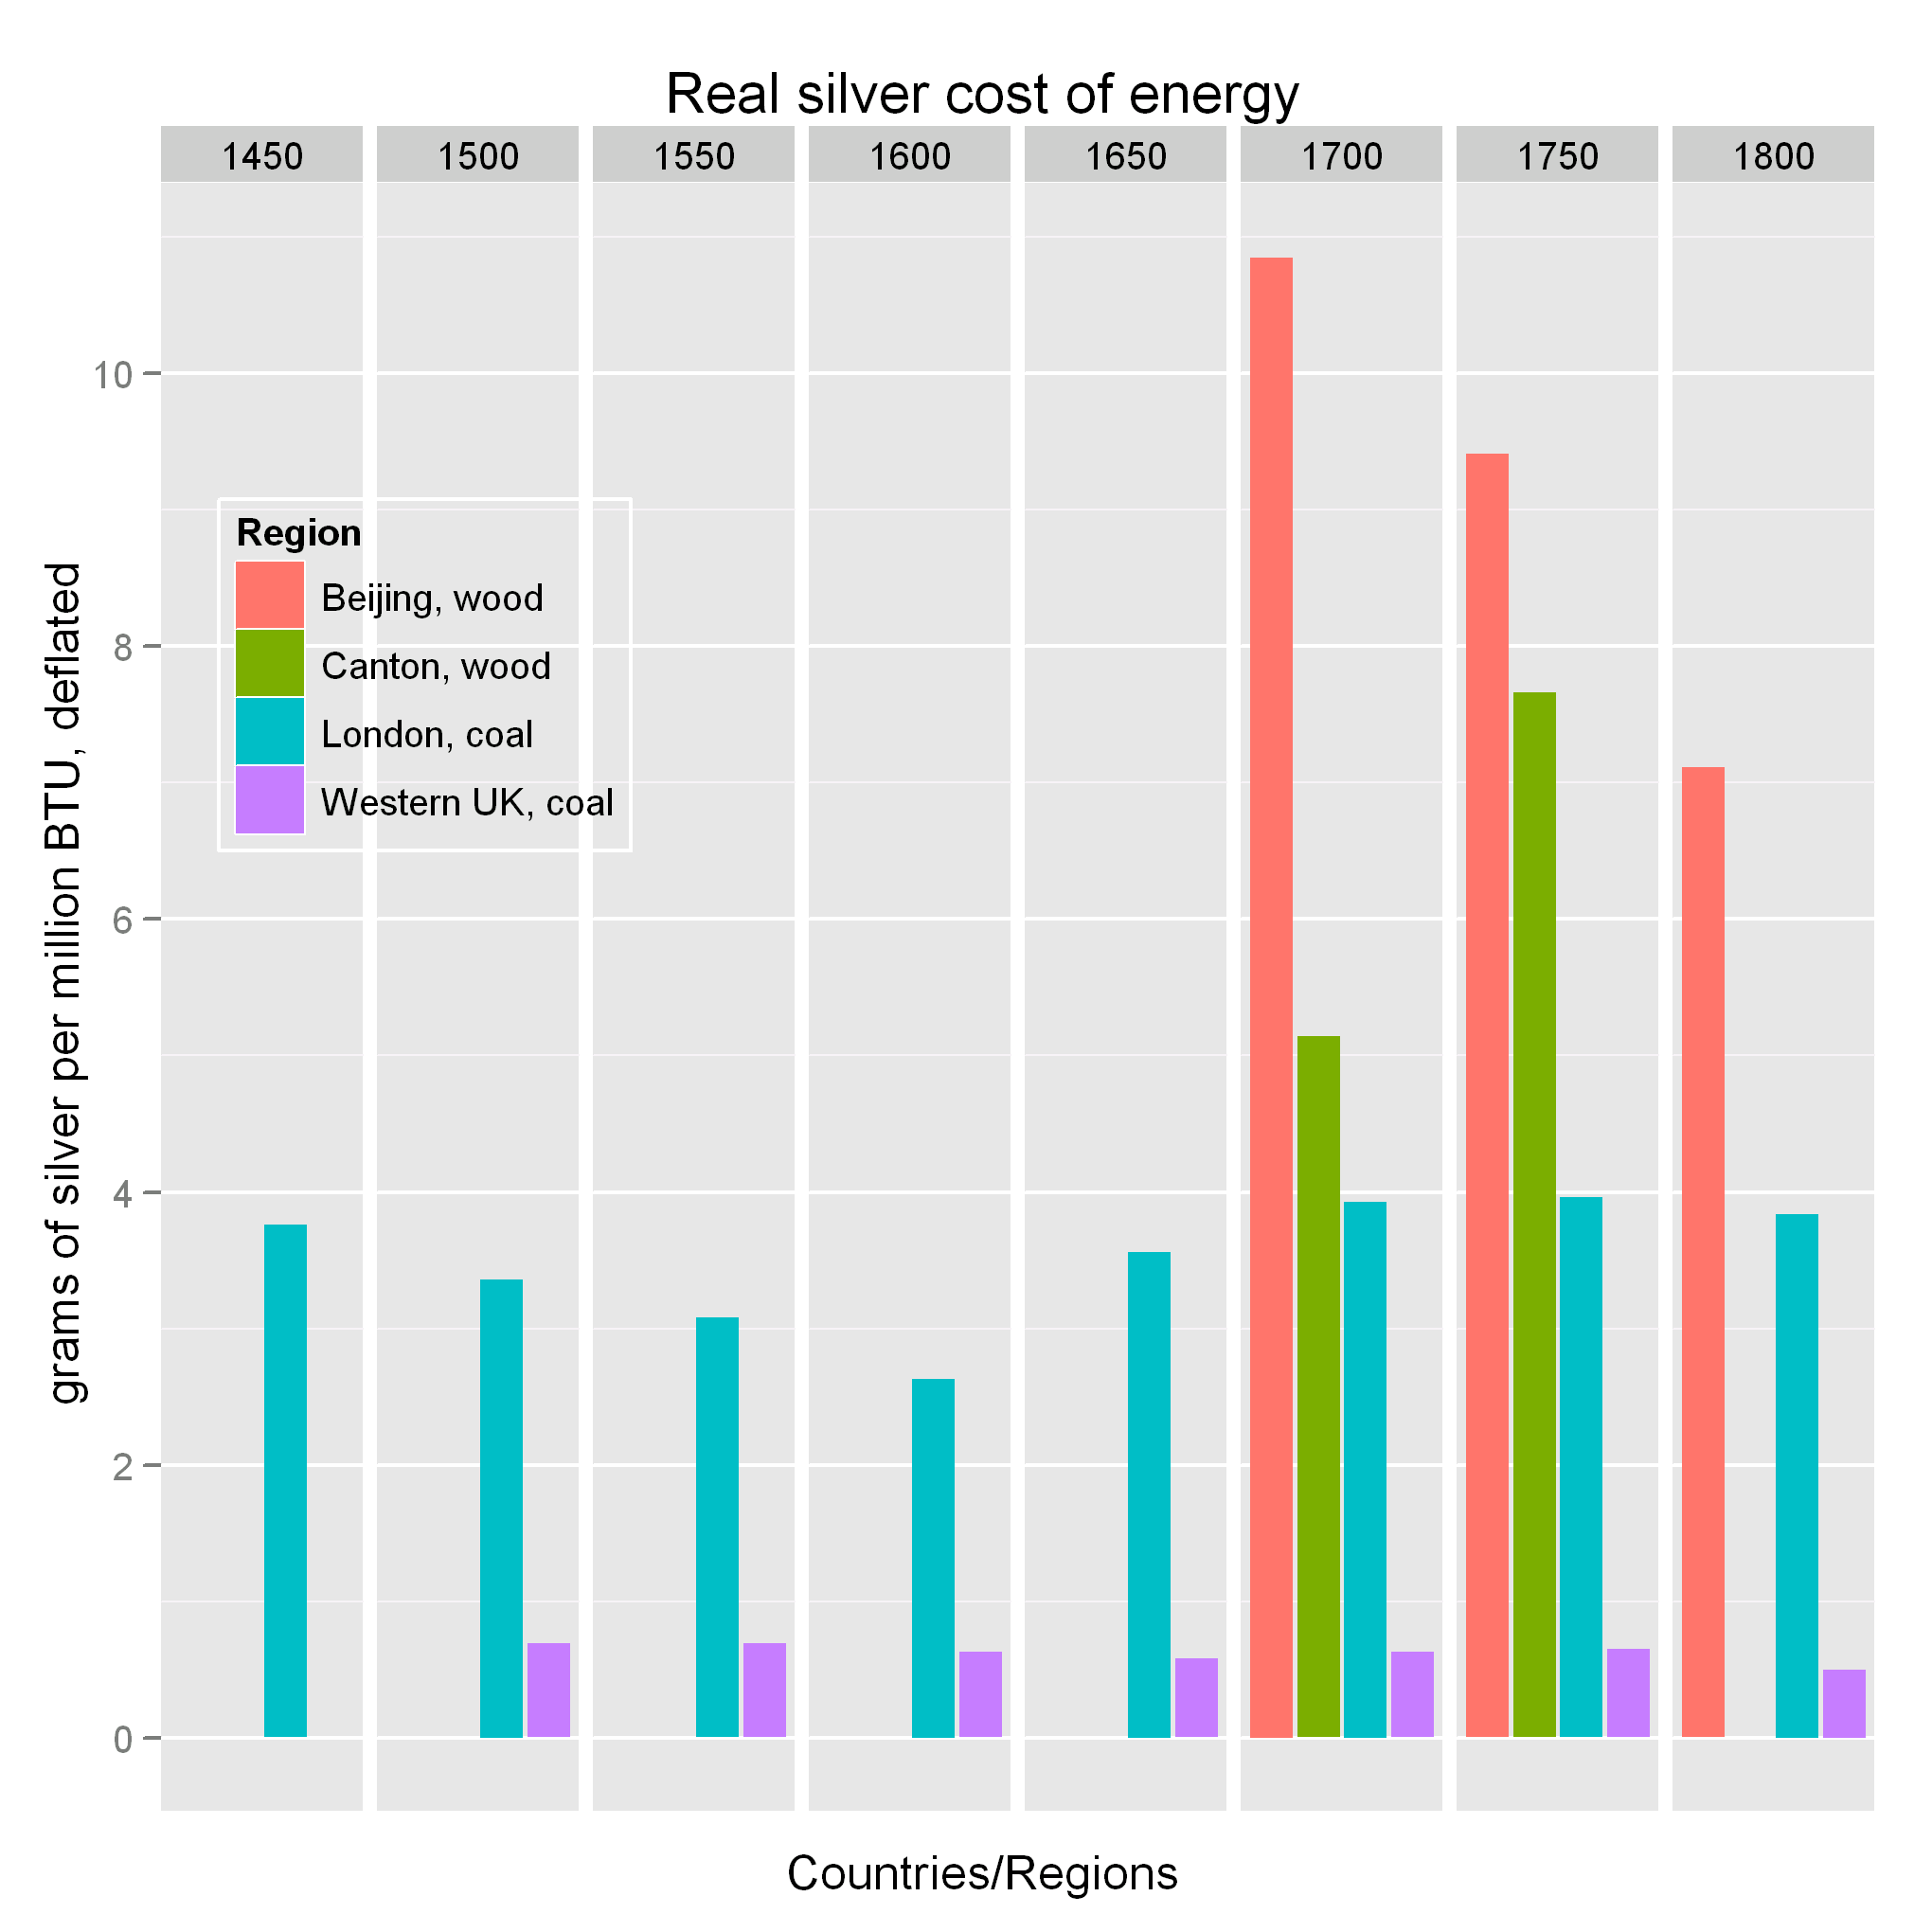
\includegraphics[width=0.39\textwidth]{/gworldenergycost.png}}
		\mbox{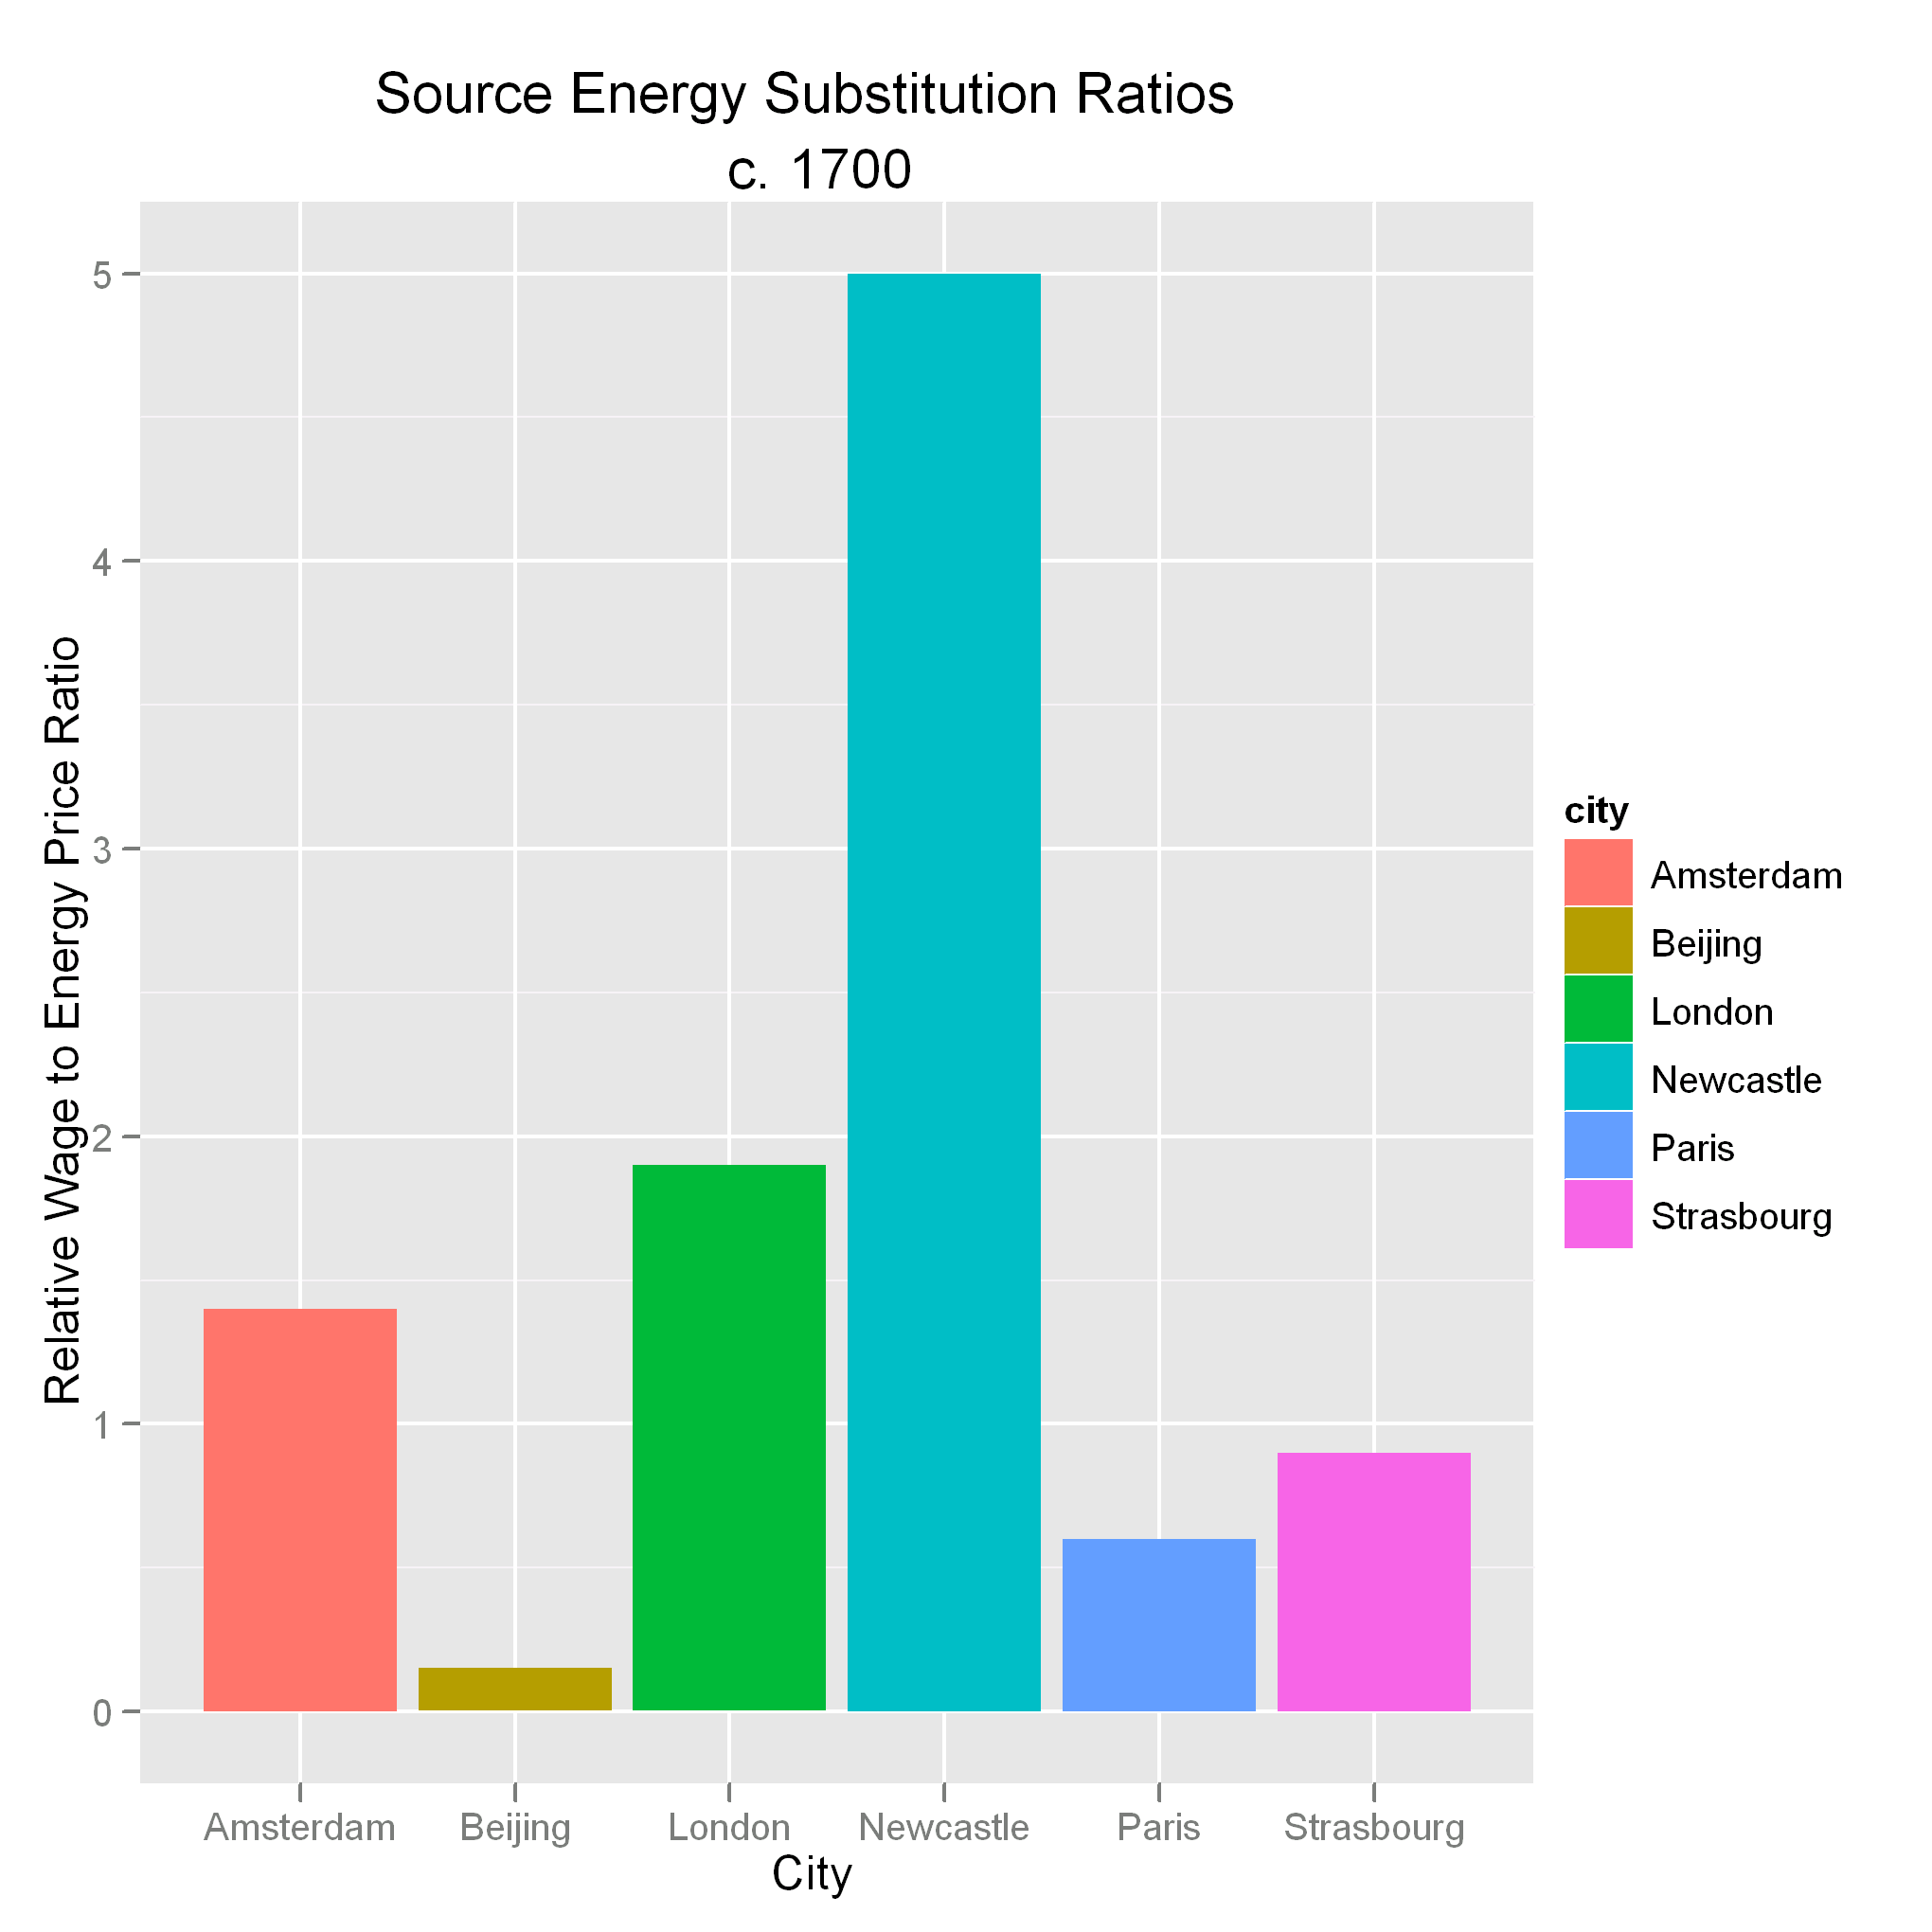
\includegraphics[width=0.39\textwidth]{wage-energy.png}}
		}
		\caption{Robert Allen, world wage and energy costs}
		\end{figure}
\end{frame}	

\subsection{Incentives for induced innovation: microeconomics 101}
\begin{frame}
\frametitle{Input substitution incentive facing inventors, entrepreneurs, Capitalists in, say, joules}
		\begin{equation*}
		\left(\frac{\small{\text{Marginal Revenue Product}}}{\small{\text{Price}}}\right)_{\tiny{\text{organic}}} =\left( \frac{\small{\text{Marginal Revenue Product}}}{\small{\text{Price}}}\right)_{\tiny{\text{mineral}}}
		\end{equation*}	
\end{frame}

\subsection{Modern economic growth -- emergent macro-level properties}

\begin{frame}
\frametitle{Energy consumption and modern economic growth} 	
 		\begin{figure}
		\centerline{
		\mbox{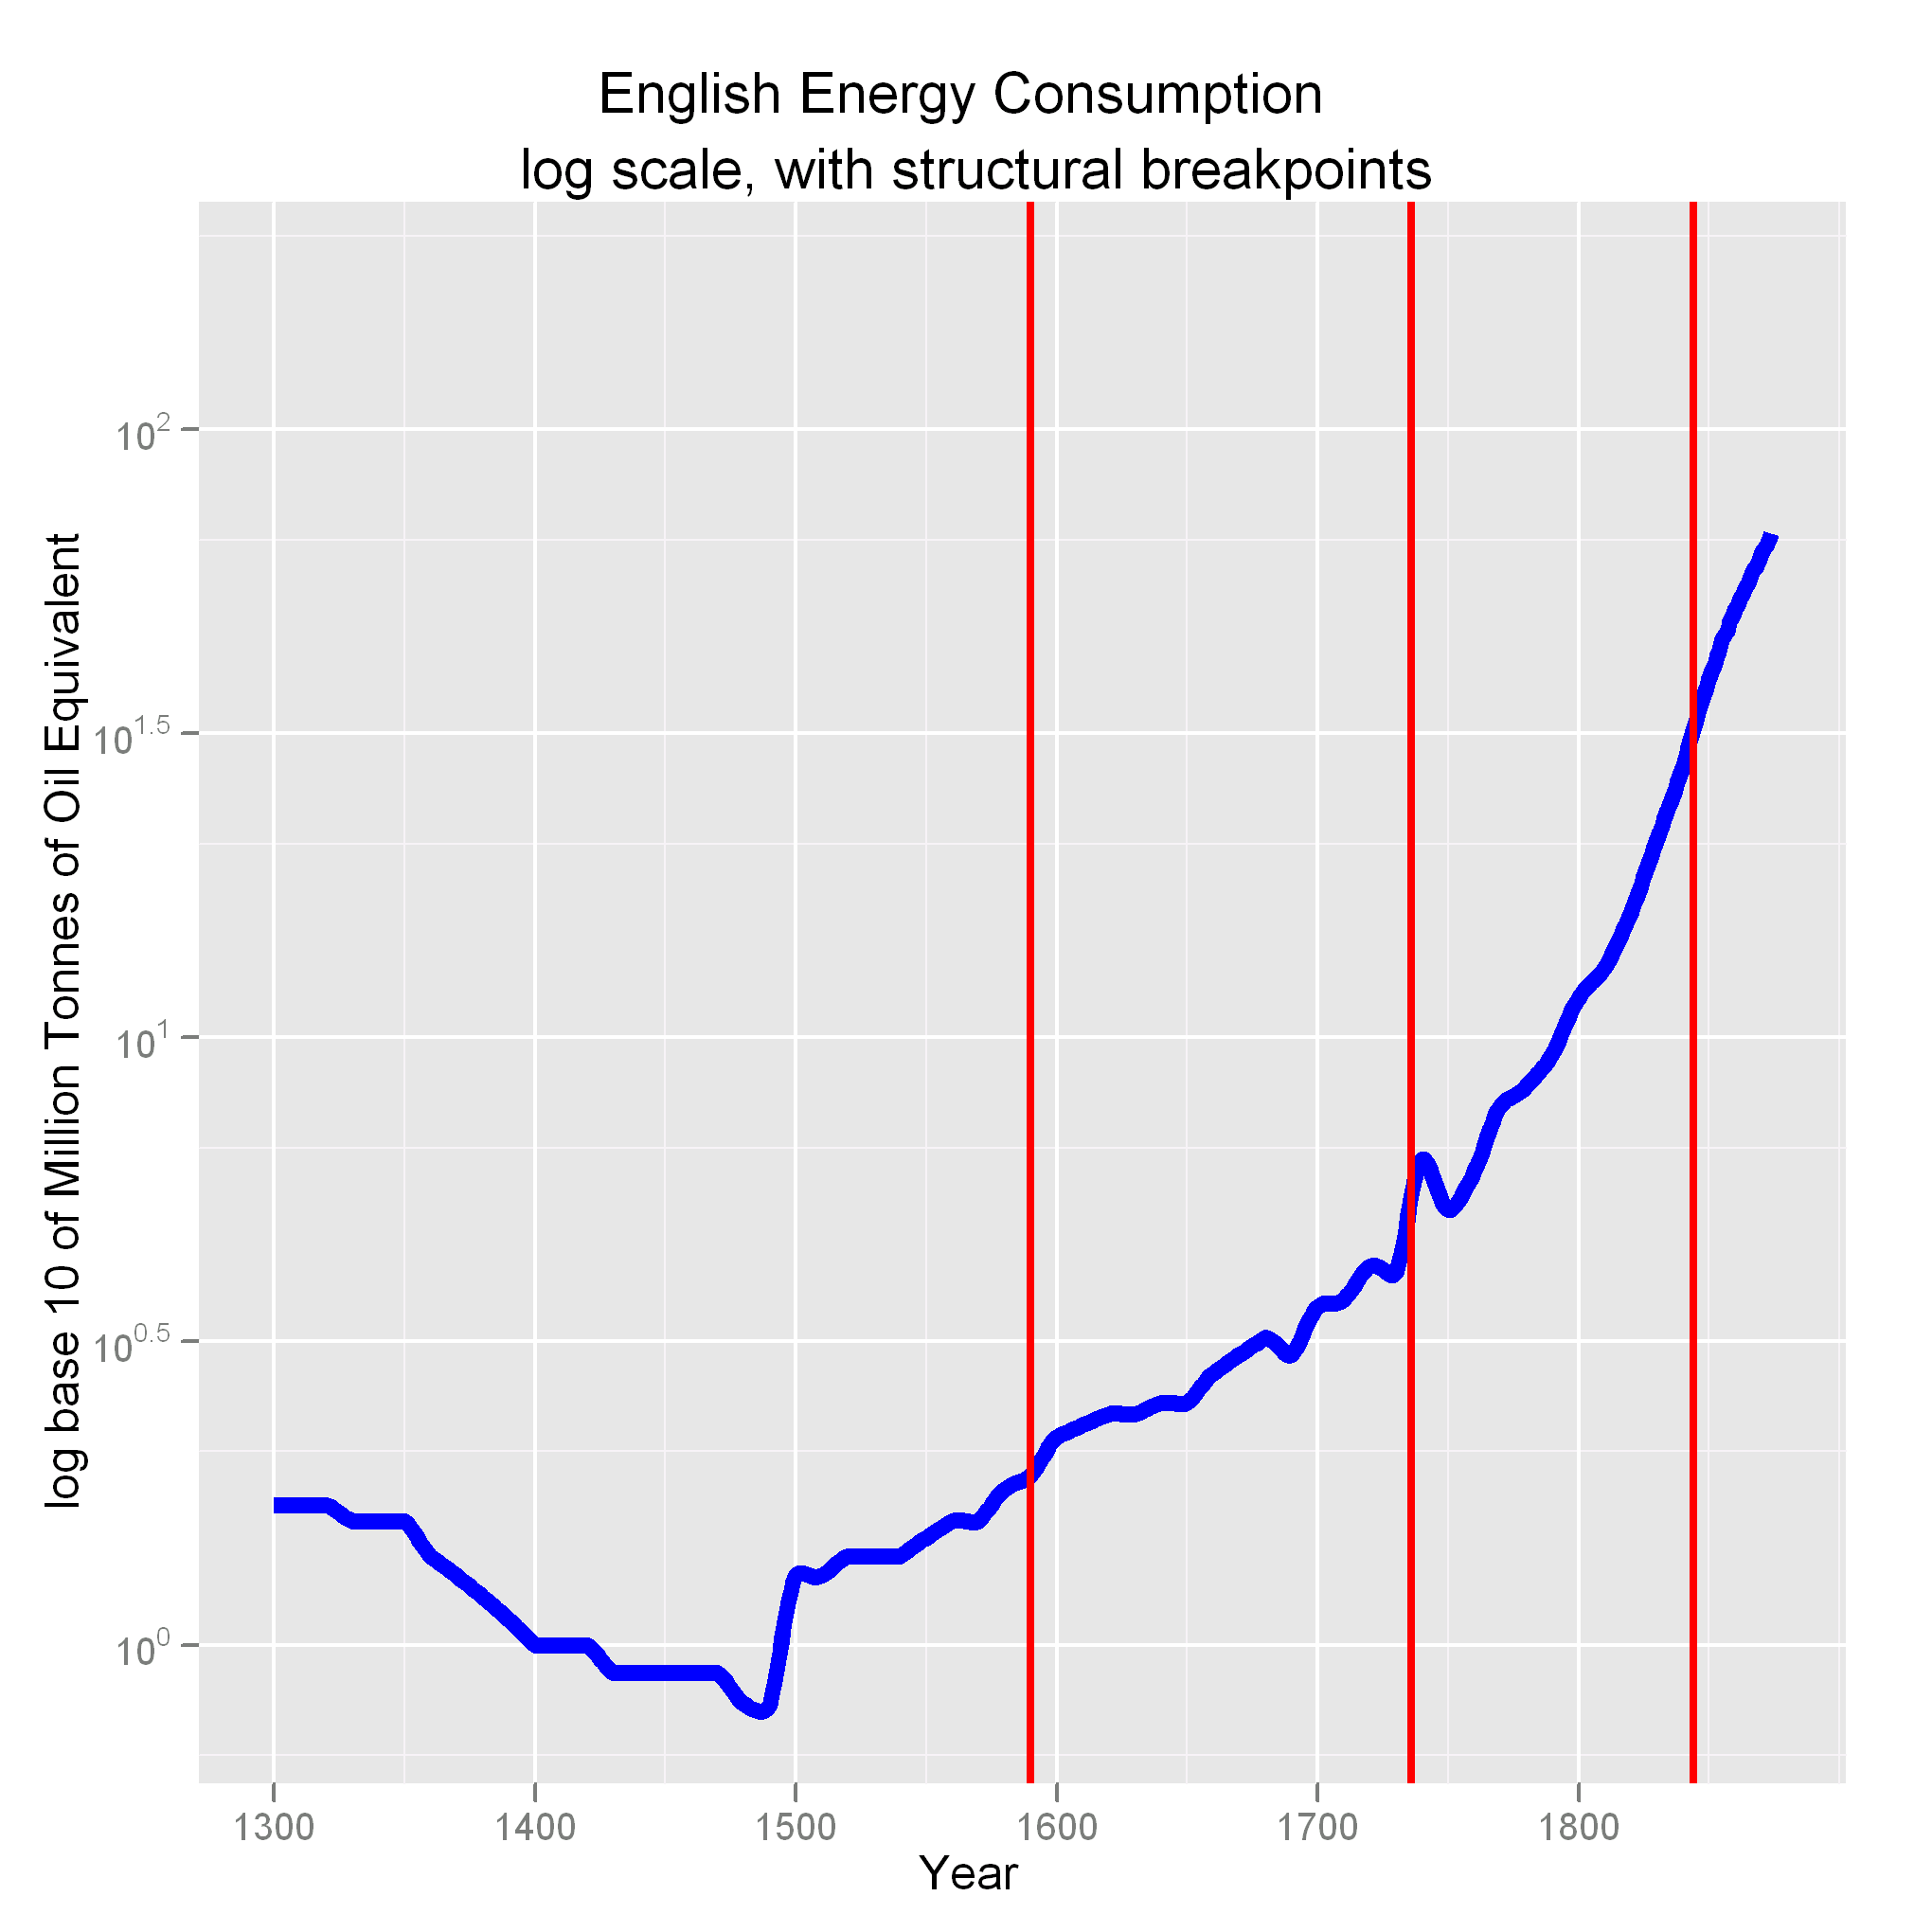
\includegraphics[width=0.39\textwidth]{gbpmtoelog.png}}
		\mbox{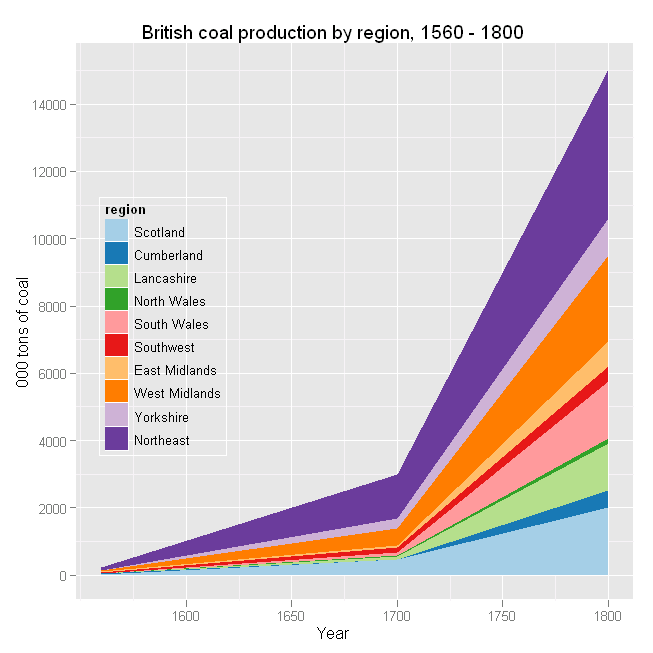
\includegraphics[width=0.39\textwidth]{allen_coal.png}}				
		\mbox{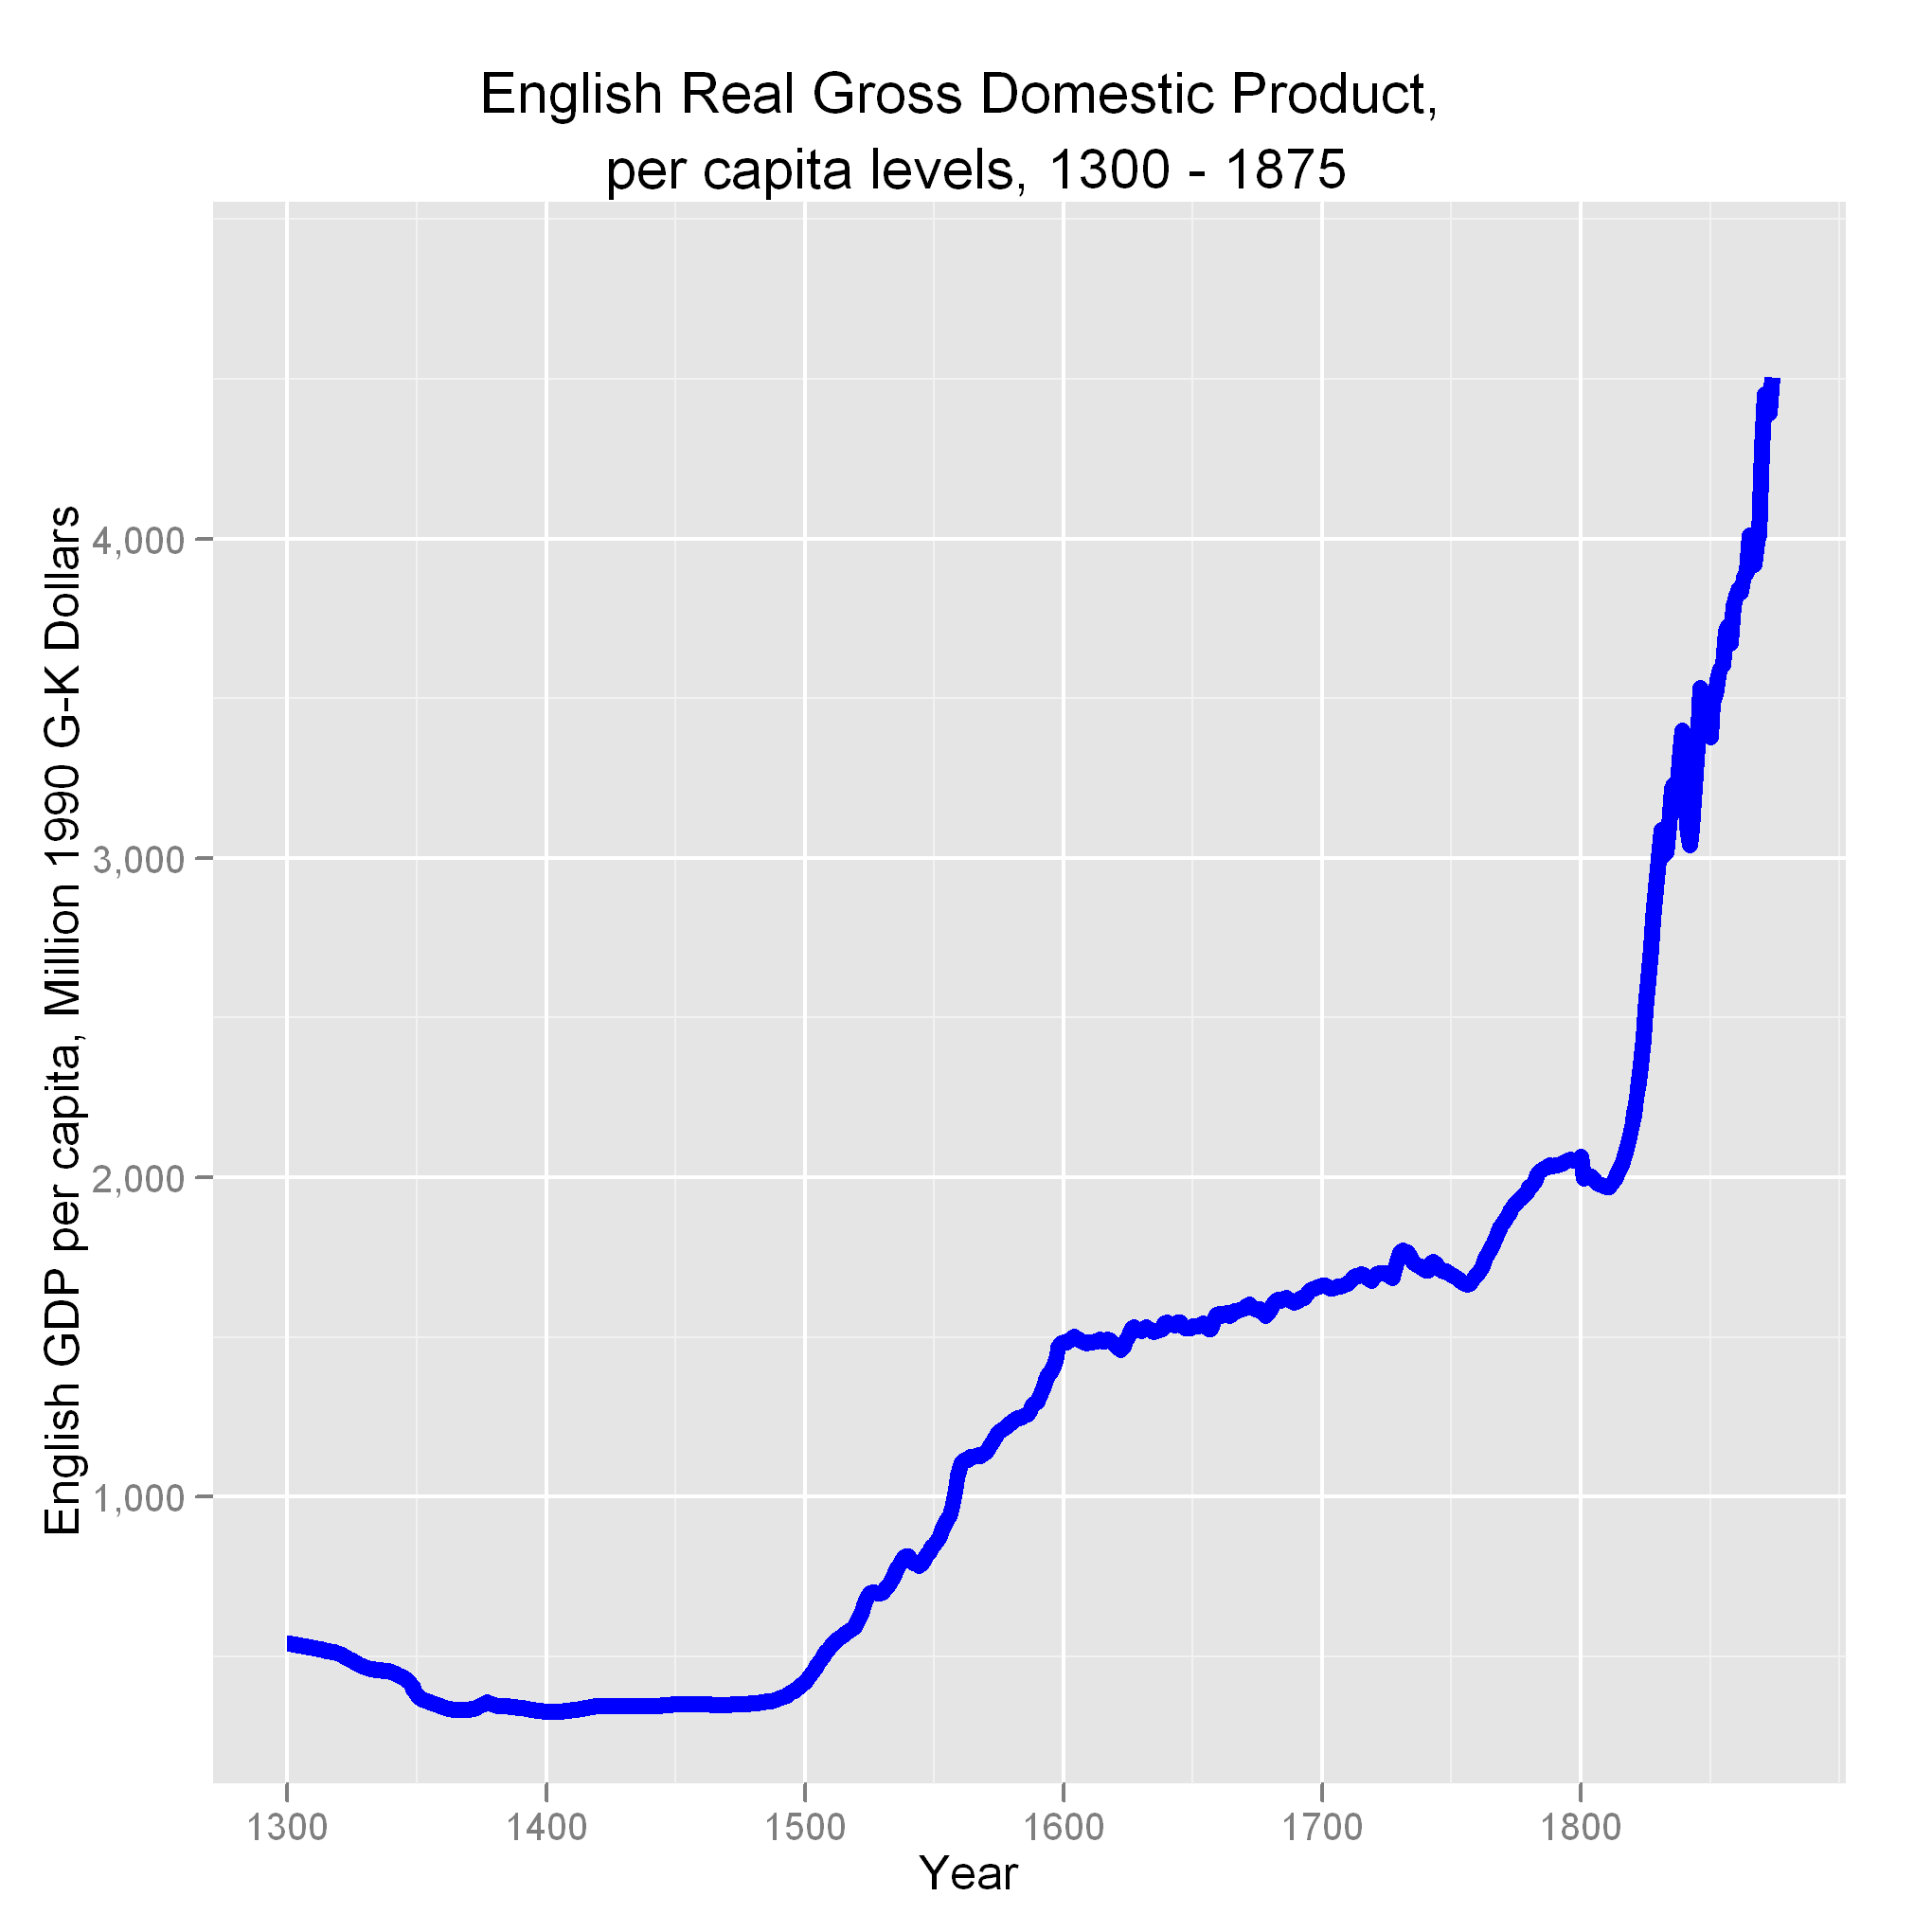
\includegraphics[width=0.39\textwidth]{/ggdppop.png}}
		}
		\caption{Roger Fouquet, energy; Allen, coal, GDP/capita constructed}
		\end{figure}
\end{frame}	

\subsection{Learning to consume energy}
\begin{frame}
 	\begin{table}[htb]
	\centering
	

	\begin{tabular}{lrrrr}
	\hline
	Year&England&China&Netherlands&India\\
	\hline \hline
	1650$^a$&&&0.63&  \\
	1820&0.61&&&\\
	1840$^a$ &&&0.33& \\
	1870&2.21&\\
	1970$^a$ &&&8.07&0.33 \\
	1973&&0.48&&\\
	1998$^b$&6.56&1.18\\
	2008$^b$&5.99&2.56&9.86&  \\
	\hline
	\end{tabular}
	\caption{Per Capita Primary Energy Consumption,	annual Tonnes of Oil Equivalent. \textit{Source:} Angus Maddison, $^a$de Zeeuw, $^b$US DOE EIA}
	\label{tab:maddison_energy}

	\end{table}
\end{frame}	

\subsection{Macro outcome and importance of the mineral energy revolution}	
 	
\begin{frame}
 		\begin{figure}
		\centerline{
		\mbox{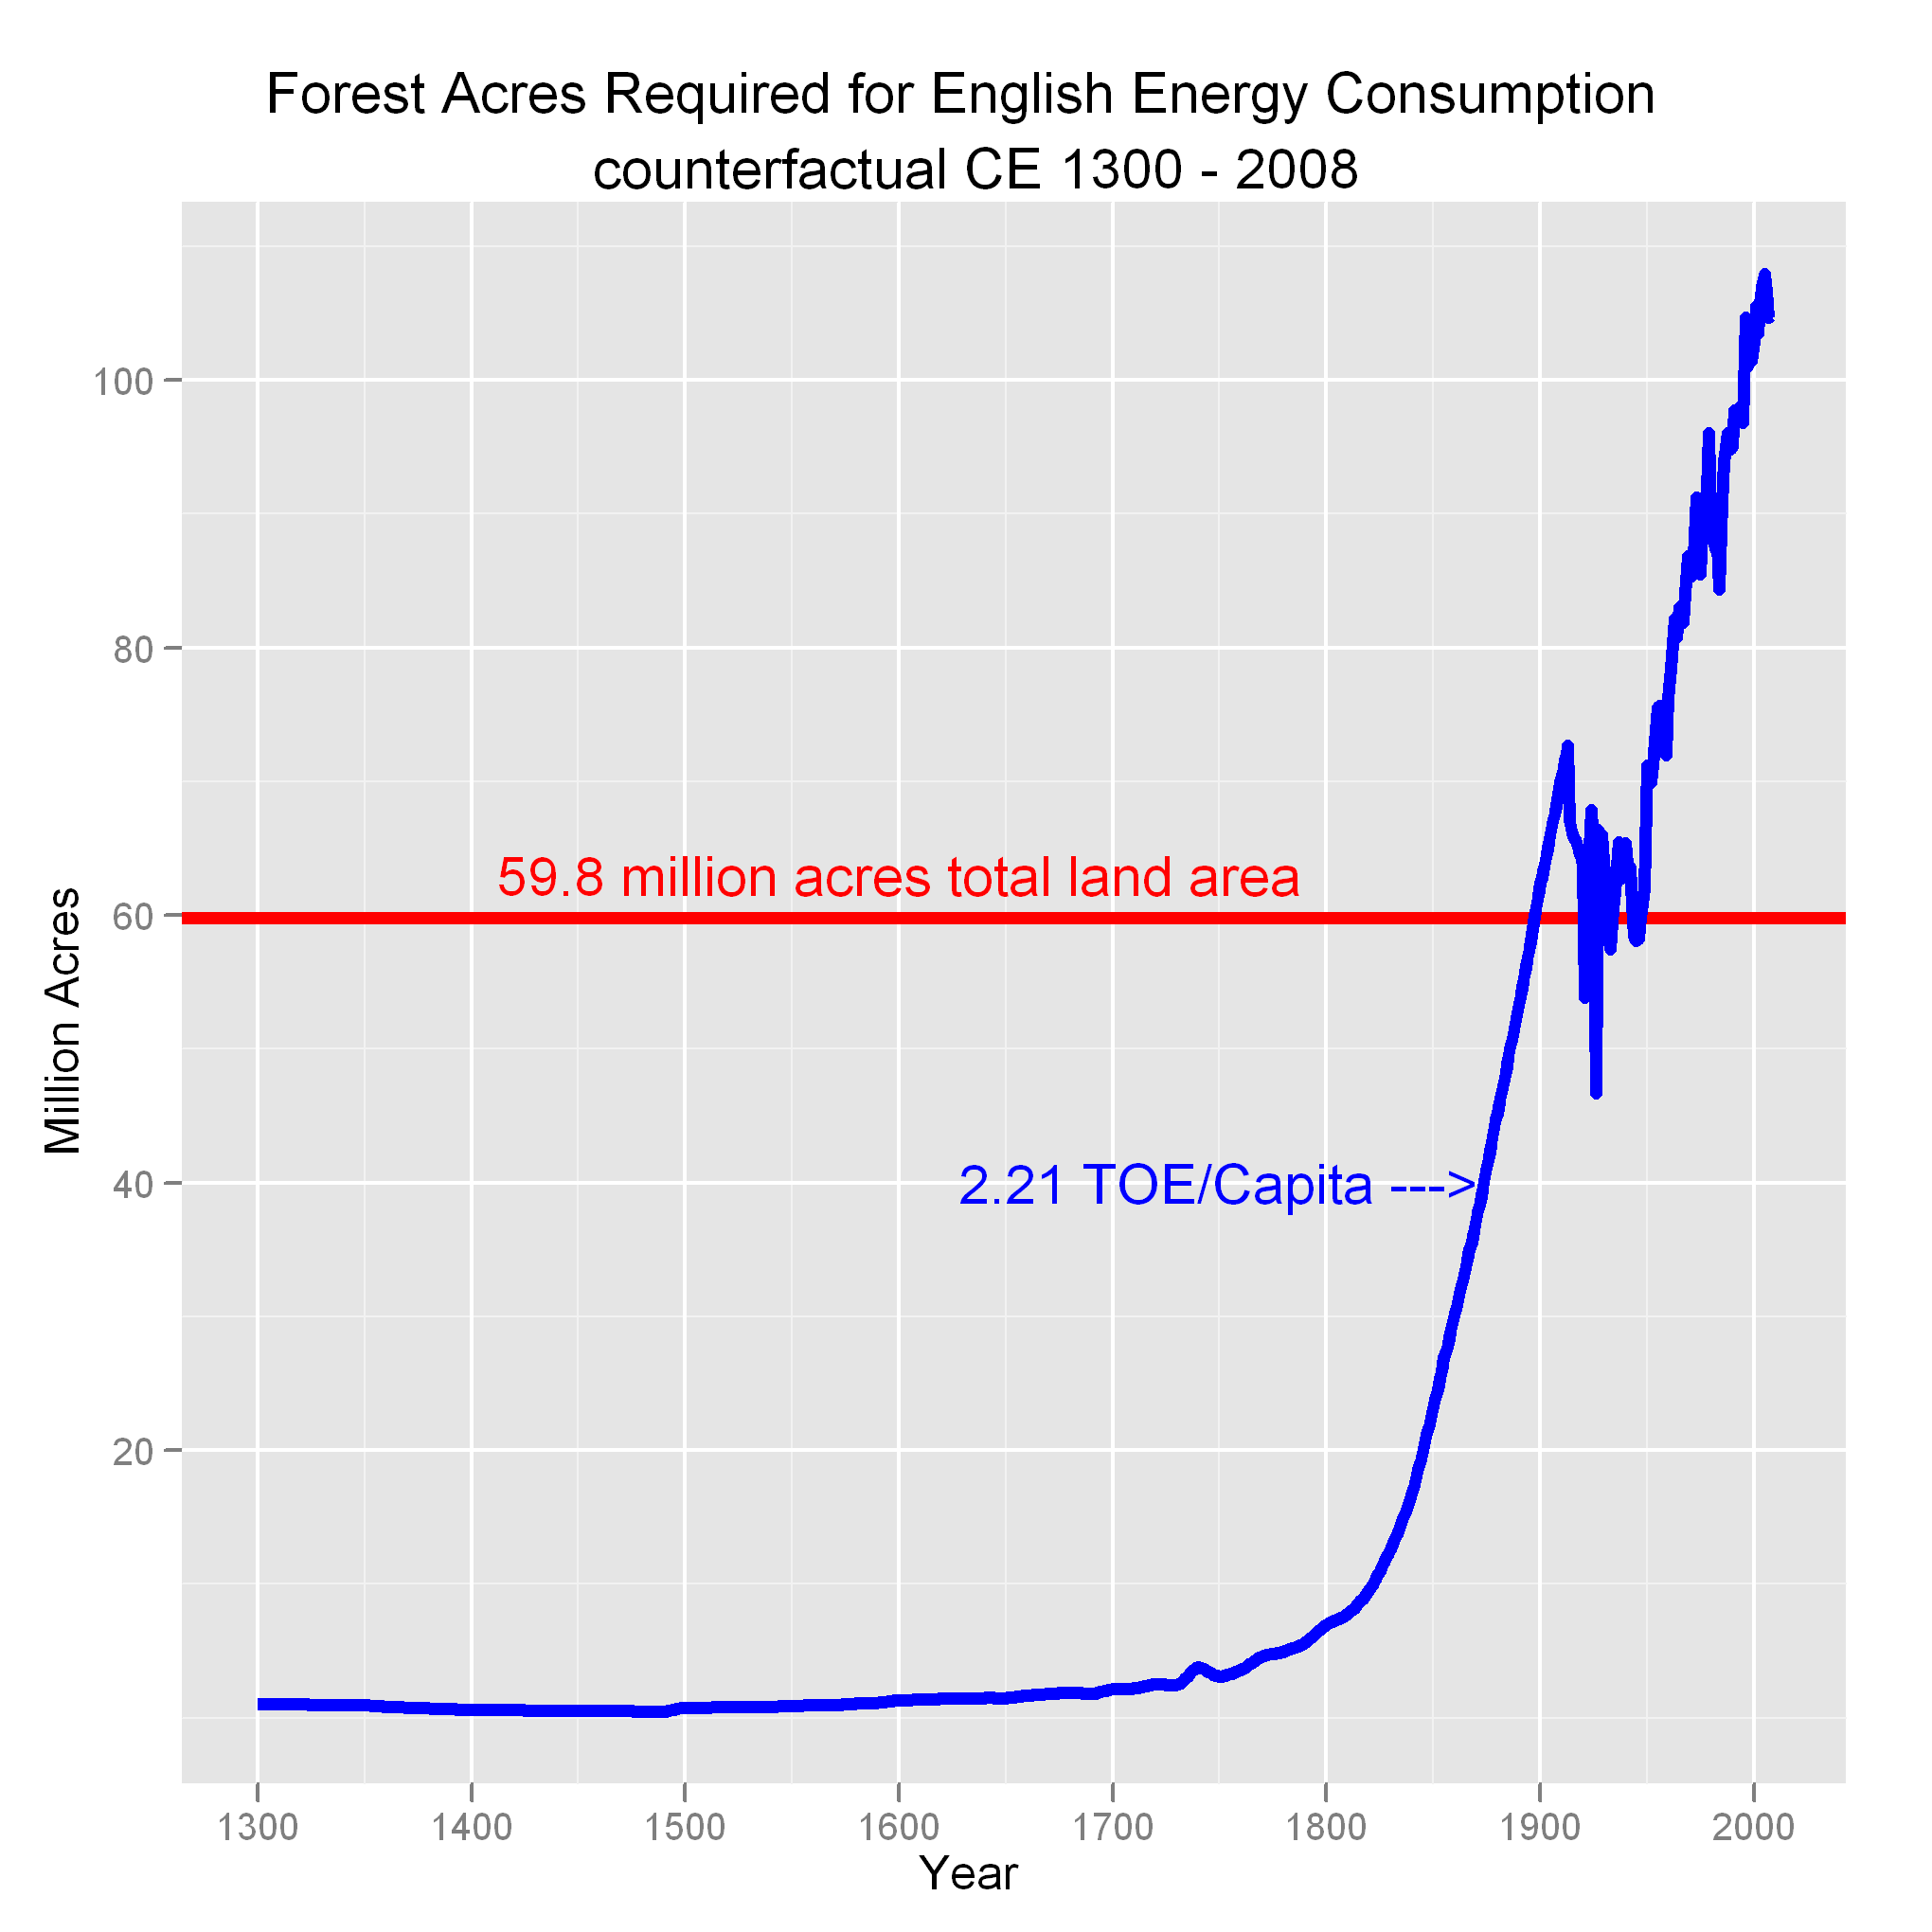
\includegraphics[width=0.58\textwidth]{wood.png}}
		\mbox{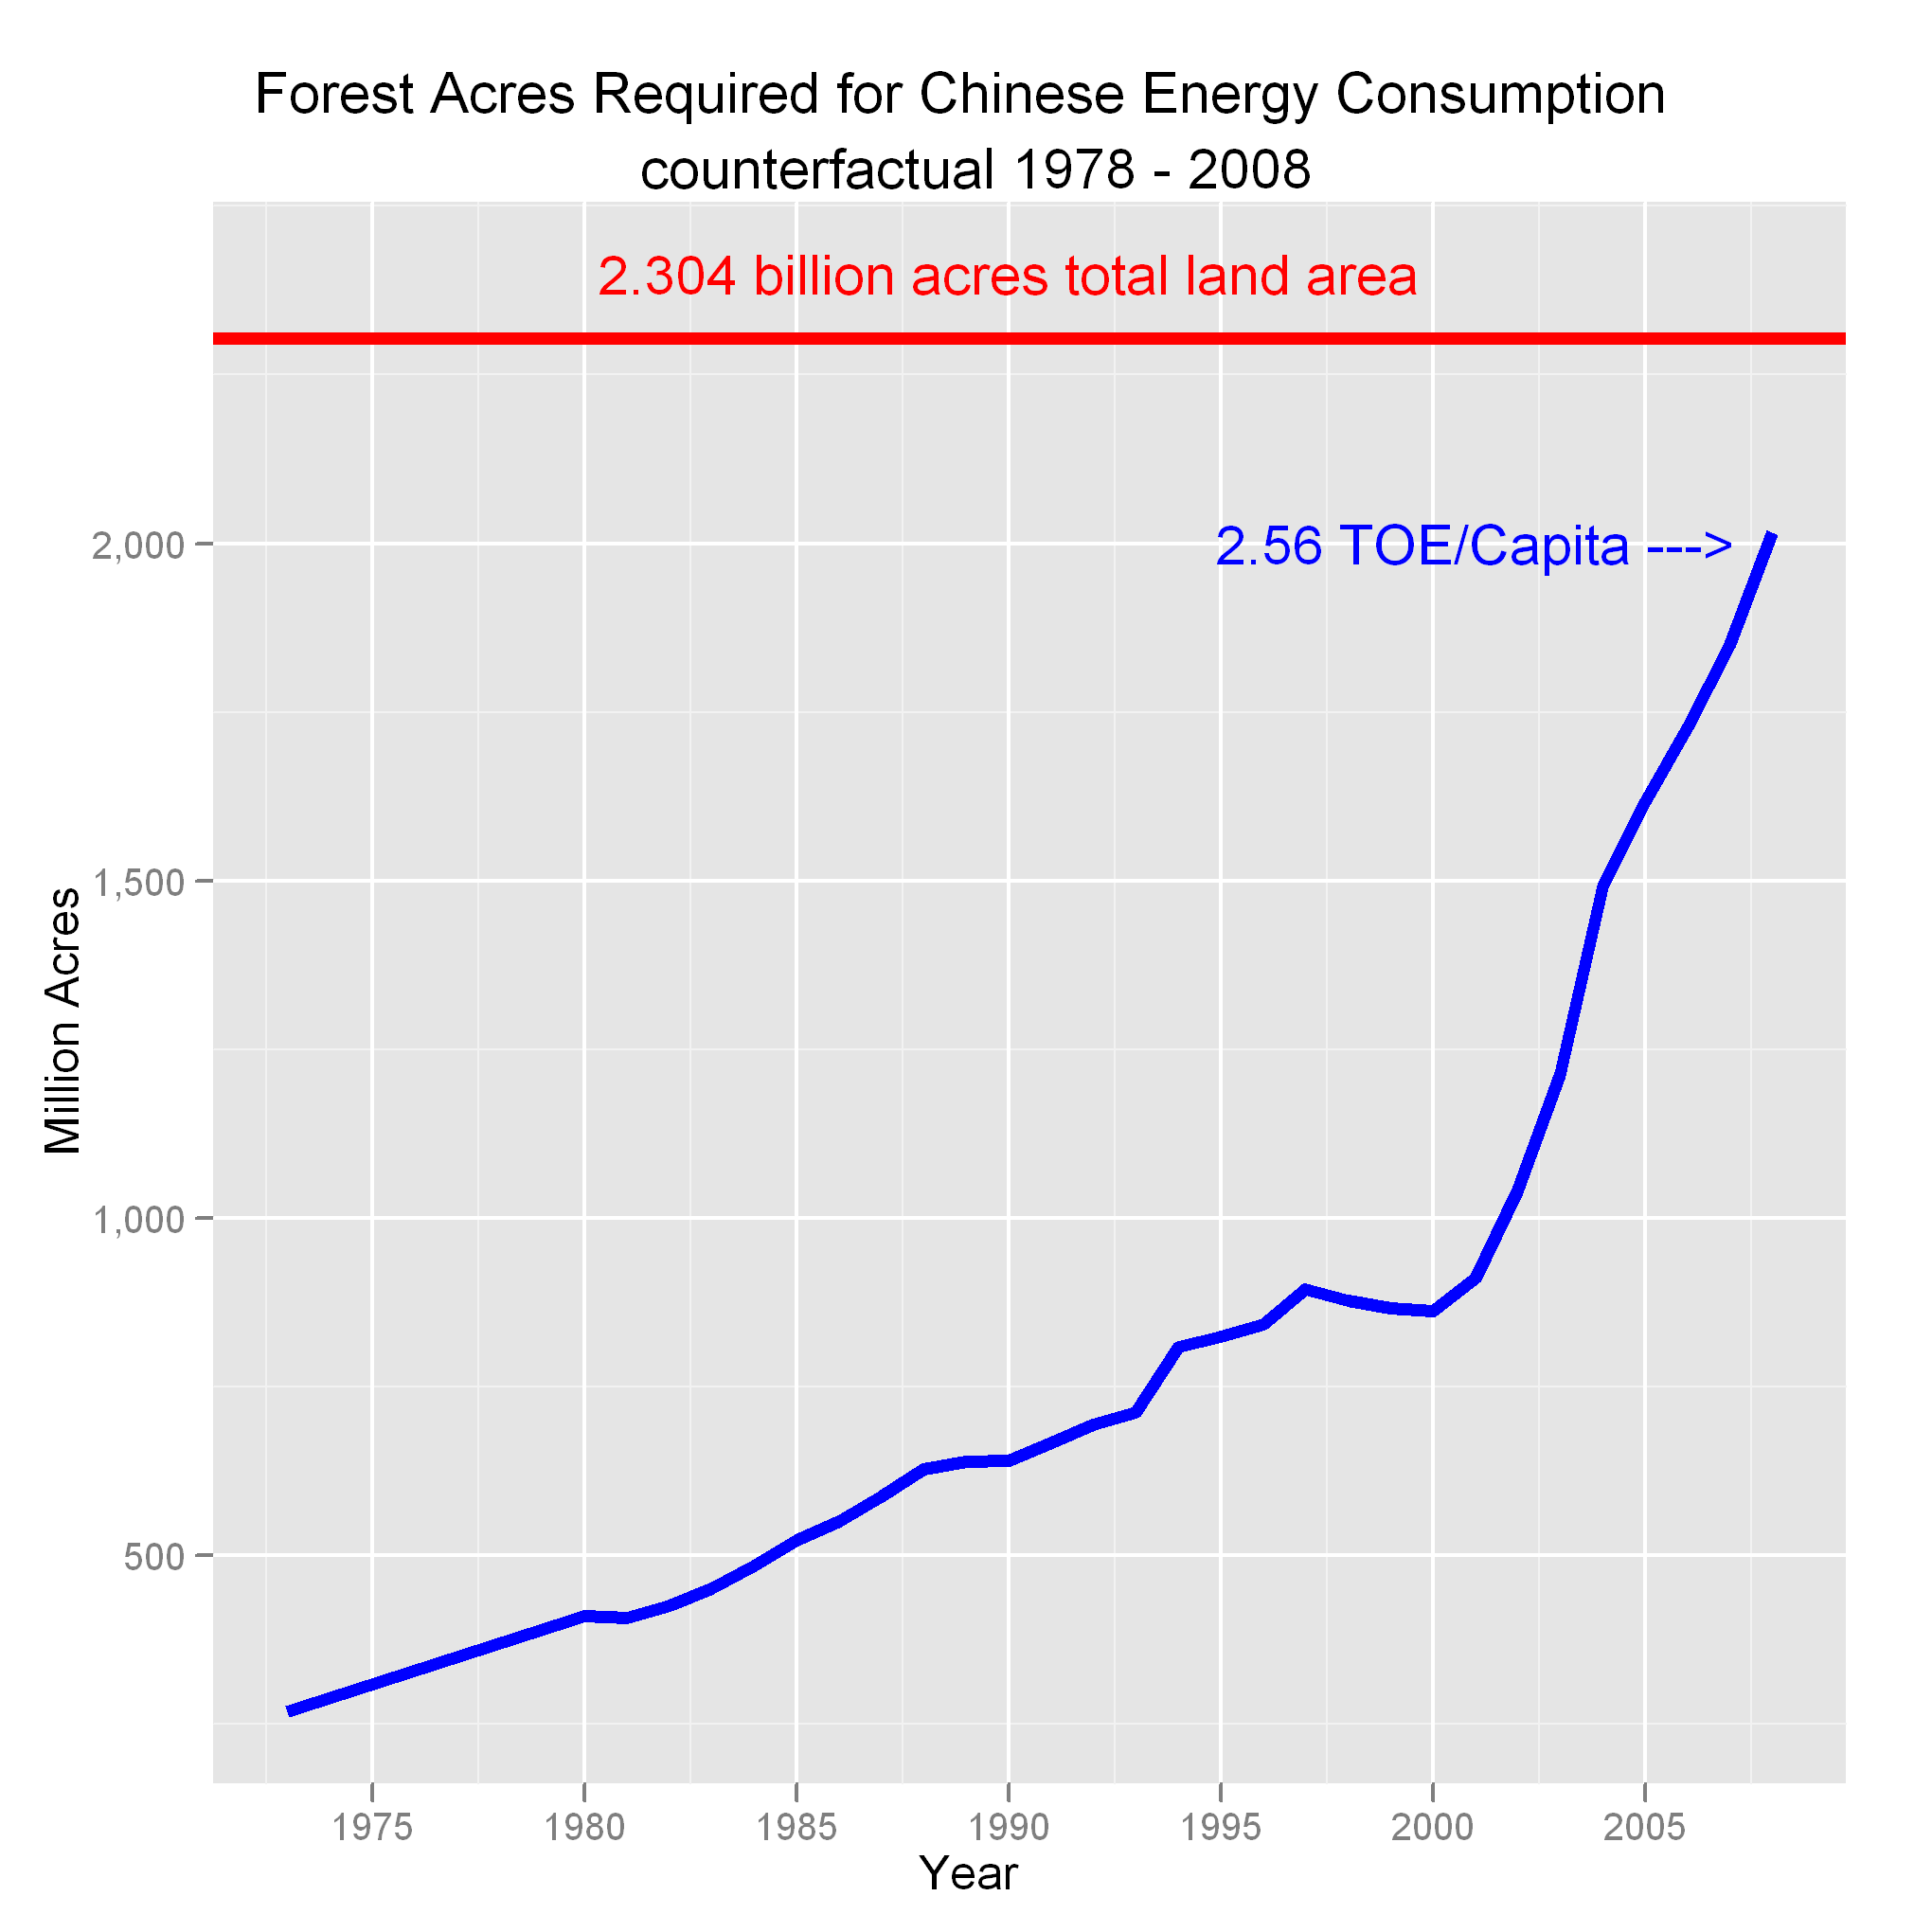
\includegraphics[width=0.58\textwidth]{chinawood.png}}
		}
		\caption{data: Fouquet, DOE, author's calculations}
		\end{figure}
\end{frame}

\begin{comment}
\begin{frame}
	
		\begin{figure}[ftb]
		\centering
		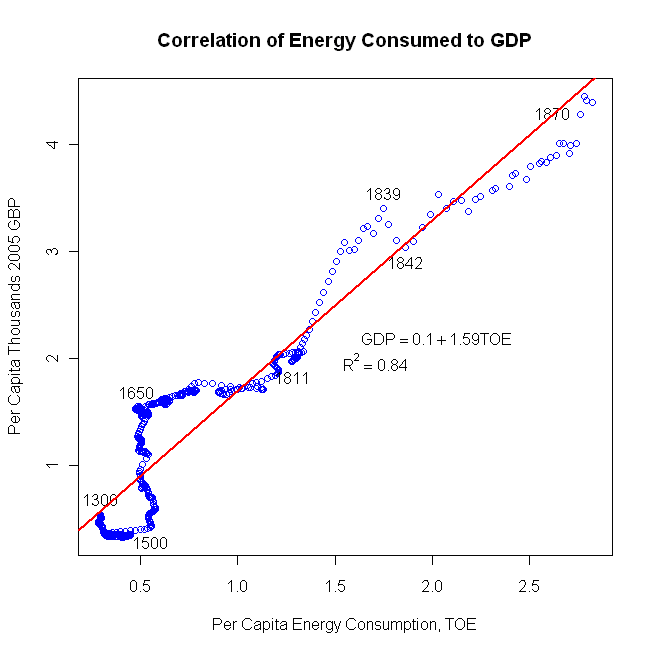
\includegraphics[width=0.7\textwidth]{corr.png}
		\caption{English energy consumption. \textit{Sources:} Roger Fouquet's energy consumption, several population sources, author's calculations.} 
		\label{fig:corr}
		\end{figure} 		
				
\end{frame}
\end{comment}

\section{Closing}

\subsection{Closing}

\begin{frame}
\begin{itemize}
%\item Microeconomic incentives existed in England sufficient to create an energy revolution and resulted in a ``virtuous'' macroeconomic feedback cycle -- the Industrial Revolution.
\item England, with great geographical and geological luck, had sufficient microeconomic incentives to create an energy revolution that resulted in a ``virtuous'' macroeconomic feedback cycle -- the Industrial Revolution.
%\item This result was at least partially dependent on geological and geographical luck, with little or no relation to any putative English institutional exceptionalism.
\item China had no comparable incentives -- had insufficient microeconomic incentives -- hence had no modern economic growth.
\item The institutions we notice, including Industrial Capitalism, appear to be induced by the economics, as usual.
\end{itemize}
\end{frame}

\begin{comment}
\begin{frame}
\begin{itemize}
\item English institutional exceptionalism or geographical and geological luck?
\pause
\item Bob Allen says armed long distance trade success and coal were the key factors for England
\pause
\item Ken Pomeranz and R. Bin Wong make the revisionist argument that Chinese institutions were functionally at least equivalent of British/European
\pause
\item and that Chinese standards of living, at least in the Yangzi Delta, were equivalent to England in 1800, so a large region had demand
\pause
\item China did not have readily accessible cheap coal, so did not undergo an energy transition
\pause
\item and so hit ecological barriers preventing modern economic growth until a late $20^{th}$ century energy transition
\end{itemize}
\end{frame}
\end{comment}

\end{document}


the varian quote from rattle
deductive vs. inductive
popper vs kaldor -- not really. 
what has changed in econometrics is that, compared to the golden age of theory (take your pick) we have enormous quantities of data and enormously powerful tools. perhaps dangerously so.
